\documentclass[a4paper, 12pt]{article}
\usepackage[utf8]{inputenc}
\usepackage[T1]{fontenc}
\usepackage[french]{babel}
\usepackage{float}

%Pour ne pas afficher les warning

% Pour utiliser la font Fira
\usepackage[sfdefault,scaled=.85]{FiraSans}
\usepackage{newtxsf}

% Pour créer des tableaux
\usepackage{array}
\usepackage{makecell}

% Pour créer des graphiques
\usepackage{tikz}
\usepackage{caption}
\usepackage{subcaption}

% Pour des environement pour le code
\usepackage{listings}

%\DeclareUnicodeCharacter{202F}{FIX ME!!!!}

\lstdefinelanguage{shell}{
    numbers=none, % --- Masque les numéros de ligne
    numberstyle=\small,
    frame=single, % Active le cadre
    frameround=tttt, % Rend les coins du cadre arrondis (t : true, f : false)
    rulecolor=\color{black},
    showspaces=false,
    showtabs=false,
    breaklines=true,
    postbreak=\raisebox{0ex}[0ex][0ex]{\ensuremath{\color{gray}\hookrightarrow\space}},
    breakatwhitespace=true,
    basicstyle=\ttfamily\small,
    upquote=true,
    % --- Définition des styles pour le shell
    keywordstyle=\color{string}, % --- Appliqué aux mots-clés (ici, utilisé pour les sections de conf)
    stringstyle=\color{string}, % --- Appliqué aux chaînes de caractères
    identifierstyle=\color{black}, % --- Appliqué aux identificateurs (noms de variables, etc.)
    commentstyle=\color{gray}, % --- Appliqué aux commentaires (pas directement utile ici, mais ajouté pour complétude)
    % --- Mots-clés pour les sections de configuration (comme [Interface], [Peer], etc.)
    keywords={Interface, Peer, PrivateKey, PublicKey, Address, ListenPort, AllowedIPs},
    % --- Caractères spéciaux
    literate=
     {*}{{*}}{1} % --- Étoile (pour les wildcard, etc.)
     {>}{{{\color{delim}{>}}}}{1} % --- Symbole "supérieur à"
     {<}{{{\color{delim}{<}}}}{1} % --- Symbole "inférieur à"
     {=}{{=}}{1} % --- Symbole "égal"
     {[}{{{\color{delim}{[}}}}{1} % --- Crochet ouvrant
     {]}{{{\color{delim}{]}}}}{1}, % --- Crochet fermant
}

\lstdefinelanguage{json}{
    numbers=none,
    frame=none, % Active le cadre
    rulecolor=\color{black},
    showspaces=false,
    showtabs=false,
    breaklines=true,
    postbreak=\raisebox{0ex}[0ex][0ex]{\ensuremath{\color{gray}\hookrightarrow\space}},
    breakatwhitespace=true,
    basicstyle=\ttfamily\small,
    upquote=true,
    morestring=[b]",
    stringstyle=\color{string},
    literate=
     *{0}{{{\color{numb}0}}}{1}
      {1}{{{\color{numb}1}}}{1}
      {2}{{{\color{numb}2}}}{1}
      {3}{{{\color{numb}3}}}{1}
      {4}{{{\color{numb}4}}}{1}
      {5}{{{\color{numb}5}}}{1}
      {6}{{{\color{numb}6}}}{1}
      {7}{{{\color{numb}7}}}{1}
      {8}{{{\color{numb}8}}}{1}
      {9}{{{\color{numb}9}}}{1}
      {\{}{{{\color{delim}{\{}}}}{1}
      {\}}{{{\color{delim}{\}}}}}{1}
      {[}{{{\color{delim}{[}}}}{1}
      {]}{{{\color{delim}{]}}}}{1},
}

% Pour la biblio
\usepackage{biblatex}
\addbibresource{biblio.bib}

% Pour les reférences
\usepackage{hyperref}
\hypersetup{
    colorlinks=true,
    linkcolor=blue,
    citecolor = blue,
    linktoc=none
}
\usepackage{csquotes}

% Pour afficher les paragraphe et sous paragraphe
\usepackage{titlesec}
%\setcounter{tocdepth}{4}
%\setcounter{secnumdepth}{4}
\titleformat{\paragraph}
{\normalfont\normalsize\bfseries}{\theparagraph}{1em}{}
\titlespacing*{\paragraph}
{0pt}{3.25ex plus 1ex minus .2ex}{1.5ex plus .2ex}

% Def couleurs
\definecolor{delim}{RGB}{20,105,176}
\definecolor{numb}{RGB}{106, 109, 32}
\definecolor{string}{rgb}{0.64,0.08,0.08}

% Page titre
\usepackage{titling}
\renewcommand{\maketitlehooka}{%
\begin{center}

\includegraphics[width=0.4\textwidth]{img/ECLlogoCroped.jpg}

\includegraphics[width=0.51\textwidth]{img/thalesLOGO.png}
\end{center}
\vspace{2cm}
}

\title{Rapport de stage d'application - Thales}
\date{}
\author{Vincent CAUJOLLE}

\begin{document}
\maketitle
\newpage
\vspace*{\stretch{.6}}
\renewcommand{\abstractname}{Résumé}
\begin{abstract}
Ce document présente mon stage d'application (stage ayant eu lieu en fin de deuxième année du cursus ingénieur généraliste de l'École Centrale de Lyon) dans le groupe Thales. La première partie de ce document est consacrée à la présentation du groupe et de son fonctionnement. Ensuite, on aborde le travail que j'ai réalisé au cours des six mois de stage en détaillant les différentes missions qui m'ont été confiées. Enfin, on trouve en fin de rapport un bref passage sur l'impact de ce stage sur la construction de mon projet professionnel (cette partie peut être absente si vous n'êtes pas de l'ECL).
\end{abstract}
\vspace{1cm}
\renewcommand{\abstractname}{Abstract}
\begin{abstract}
This document presents my application internship (internship that took place at the end of the second year of the general engineering curriculum at École Centrale de Lyon) within the Thales group. The first part of this document is dedicated to the presentation of the group and its operation. Then, we discuss the work I carried out during the six months of internship, detailing the various missions given to me. Finally, a brief passage on the impact of this internship on the construction of my professional project can be found at the end of the report (this part might not be present if you are not from the ECL).
\end{abstract}
\vspace*{\stretch{1}}
\newpage
\tableofcontents
\newpage
\listoffigures
\listoftables
\newpage

\section*{Glosaire}
\begin{enumerate}
\item \textbf{GBU}\label{GBU}: Une Global Business Unit est une division du groupe Thales se concentrant sur un marché spécifique
\item \textbf{XOR}\label{XOR} ($\oplus$):\\
	\begin{table}[h]
	\center
	\begin{tabular}{|c|c|c|}
	\hline
		$a$ & $b$ & $a\oplus b$ \\ \hline\hline
		0 & 0 & 0 \\ \hline
		0 & 1 & 1 \\ \hline
		1 & 0 & 1 \\ \hline
		1 & 1 & 0 \\ \hline
	\end{tabular}
	\caption{table de vérité du XOR}
	\label{XOR_table}
	\end{table}
\item \textbf{Byte}\label{byte}: 8 bits	
\item \textbf{American Standard Code for Information Interchange (ASCII)}\label{ASCII}: C'est un code de caractères standard utilisé pour représenter les textes en informatique et en télécommunication. L'ensemble des caractères ASCII sont codé sur 7 bits ce qui laisse dont $2^7 = 128$ caractères possibles (donc on est très limité avec l'ASCII)
\item \textbf{UTF-8}\label{utf}: Comme \hyperref[ASCII]{ASCII}, c'est un code de caractères standard utilisé pour représenter les textes en informatique et en télécommunication. Mais par contre il code ses caractères sur 1 à 4 \hyperref[byte]{byte}s selon la rareté d'utilisation du caractère. 
\item $\textbf{Gallois Field (}GF\textbf{)}$\label{GF}: En mathématiques, un corps fini ou corps de Galois est un corps qui contient un nombre fini d'éléments. L'exemple le plus courant de corps finit est $\mathbb{Z}/p\mathbb{Z}$.
\item \textbf{Diffie Hellman (DH)}\label{DH}: L'échange Diffie-Hellman est un protocole qui permet à deux parties, Alice et Bob, de partager un secret commun $K$. Le protocole repose sur la difficulté de résoudre le problème du logarithme discret. \\

\noindent Avec $p \in \mathbb{P}$ et $g\in \mathbb{Z}/p\mathbb{Z}$, Alice et Bob choisissent chacun un nombre qu'ils gardent secret et calculent de leur côté 
$$
A = g^a \lbrack n \rbrack, \quad B = g^b \lbrack n \rbrack 
$$
Alice envoie $A$ à bob et réciproquement, ensuite Alice (resp Bob) calcule $K = B^a \lbrack n \rbrack$ (resp $K = A^b \lbrack n \rbrack$) \\

\noindent En effet on a bien $A^b = g^{ab} = B^a \lbrack n \rbrack$ et comme $a$ (resp $b$) n'est connu que de Alice (resp Bob) il n'y a que Alice et/ou Bob qui peuvent retrouver ce secret $K$.\\

\noindent On remarque que ce protocole à besoin de la présence des 2 parties pour permettre l'échange (échange synchrone)	
\item \textbf{Keyed-Hash Message Authentication Code (HMAC)}\label{HMAC}: HMAC est un code d'authentification de message qui utilise une fonction de hachage
\item \textbf{Key Derivation Function (KDF)}\label{KDF}: une KDF permet de générer une clef à partir d'une donnée arbitraire. En plus de ça, une KDF doit garantir que la sortie est indépendante de l'entrée et qu'elle est "difficile" à deviner. 
\item \textbf{HMAC-based Key Derivation Function (HKDF)}\label{HKDF}: HKDF est une \hyperref[KDF]{KDF} qui utilise la fonction \hyperref[HMAC]{HMAC}.

	\item \textbf{Concaténation} ($\Vert$)\label{concat}: On ajoute bout à bout les deux suites de bits
	\item \textbf{Transmission Control Protocol (TCP)}\label{TCP}: Le TCP est un protocole de communication qui permet de transmettre des données de manière fiable et ordonnée sur un réseau. \\
Lors d'une communication TCP il y a un ping pong entre le client et le client
	\begin{figure}[h]
		\centering
		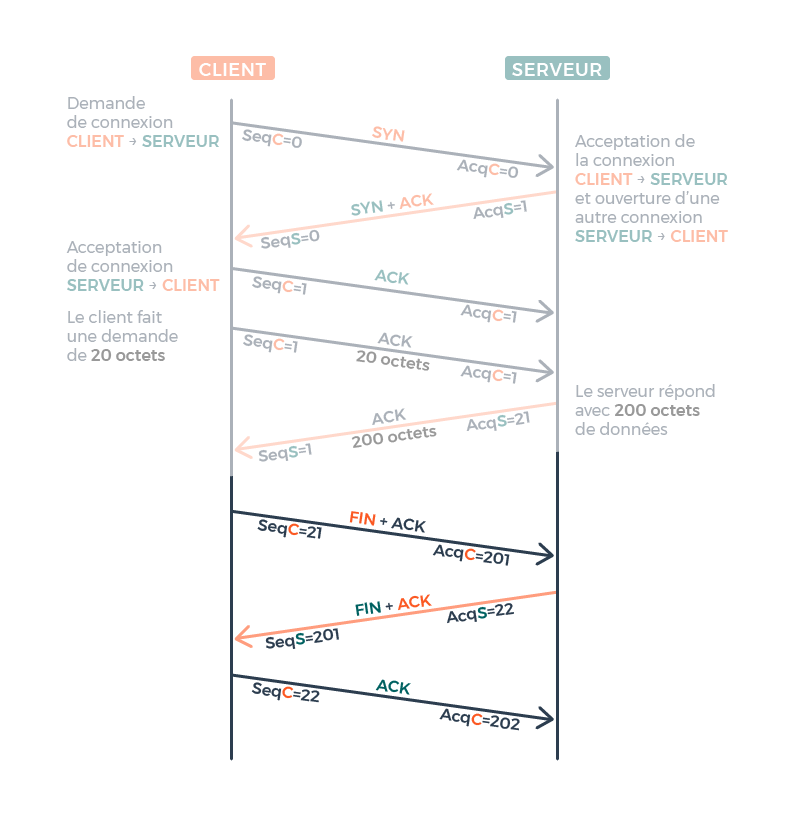
\includegraphics[width=.7\textwidth]{img/TCP.png}
		\caption{Ping pong entre le client et le serveur avec un protocole TCP}
		\label{pingpongtcp}
	\end{figure}
\item \textbf{User Datagram Protocol (UDP)}\label{UDP}: Comme pour \hyperref[TCP]{TCP}, UDP est un protocole de communication qui permet de transmettre des données mais cette fois ci de manière non fiable et sans connexion. \\
Une caractéristique importante de l'UDP dans le cadre de mon stage est qu'il n'y a pas de détection d'erreur. Ainsi, un attaquant n'aura aucun retour sur les paquets qu'il envoie au serveur UDP.
\item \textbf{Algorithmes post-quantique}\label{postquant}: Les algorithmes post-quantiques sont des algorithmes de cryptographie qui sont conçus pour résister aux attaques d'un ordinateur quantique. 
\item \textbf{National Institute of Standards and Technology (NIST)}\label{NIST}: C'est un institut de recherche et de normalisation américain. Dans le domaine de la cryptographie, le NIST joue un rôle important en définissant les standards et les recommandations pour les algorithmes et les protocoles de cryptographie utilisés pour protéger les informations sensibles. Les standards cryptographiques du NIST sont largement adoptés et respectés à l'échelle internationale, et ils ont un impact significatif sur la sécurité des systèmes d'information et des communications.
\item \textbf{Treillis}\label{treillis}: On appelle treillis tout ensemble ordonné dans lequel deux éléments quelconques ont toujours une borne supérieure et une borne inférieure
\end{enumerate}
\newpage

\section{Introduction}
Dans le cadre de ma deuxième année d'études à l'Ecole Centrale de Lyon, j'ai eu l'opportunité de réaliser un stage d'application de six mois au sein de Thales, de mai à novembre 2024. Sous la tutelle de M. Mahmoud Chilali, j'ai occupé le poste de cryptographe/développeur cryptographique. \\

Au cours de ce stage, j'ai approfondi mes connaissances en cryptographie en apprenant à maîtriser divers algorithmes de chiffrement et de signature numérique, tels que AES, RSA ou encore Ed25519. J'ai également eu l'occasion de mettre certains algorithmes à l'épreuve, en démontrant notamment la vulnérabilité du chiffrement AES en mode CBC.
Parallèlement, j'ai découvert d'autres aspects de la cryptographie, tels que la protection des données sensibles avec les modules de sécurité matériels (HSM) et d'autres sujets passionnants. \\

L'objectif principal de mon stage était de préparer le terrain pour une refonte du logiciel Sakyena en Rust, j'ai pu réécrire une grande partie de ces algorithmes dans ce nouveau langage passionnant. \\

Ce rapport présente l'entreprise qui m'a accueilli et le contexte dans lequel j'ai effectué mon stage. Ensuite, je détaille les résultats de mes travaux et les connaissances que j'ai acquises au cours de ce stage, en mettant l'accent sur les algorithmes que j'ai étudiés et programmé en Rust. Enfin, je montre l'impact de ce stage sur la construction de mon projet professionnel

\section{Contexte du stage et organisation de l'entreprise}
Dans le cadre de ma deuxième année du cycle ingénieur de l'ECL, j'ai pu faire mon stage d'application du 27/05/24 au 27/11/24 à Thales.
\subsection{Groupe Thales}
\noindent\emph{Les informations qui m'ont permis d'écrire cette sous section sont tirées de \cite{thalesgroupe}.}\\

\og{}\emph{Construisons ensemble un avenir de confiance}\fg{} est la devise de Thales. Créé en 1893, Thales, sous la direction de Patrice Caine est présent dans 68 pays, compte près de 81000 collaborateurs et affiche un chiffre d'affaire de plus de 16 milliards d'euros. \\

\begin{figure}[h]
	\centering
	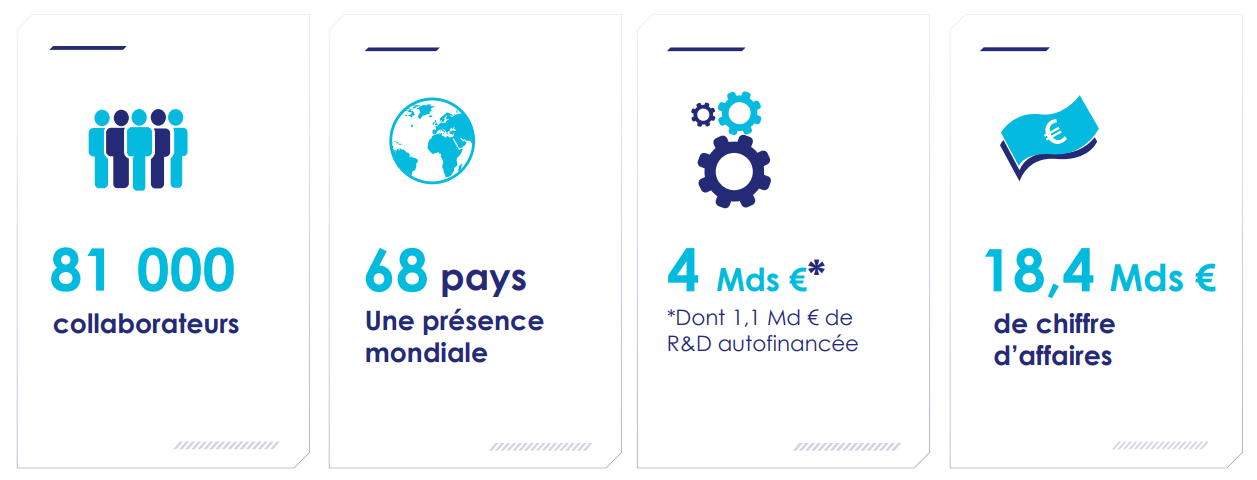
\includegraphics[width=\textwidth]{img/thales_pres.png}
	\caption{Chiffres clés de 2023 du groupe Thales}
	\label{chiffres2023}
\end{figure}

Les clients de Thales sont de grandes organisations - États, administrations, entreprises, etc. Ses clients sont responsables des opérations, des services et des infrastructures critiques de la société telles que : la défense, la sécurité, le transport aérien et ferroviaire, la banque, les télécommunications et bien d’autres.
Pour gagner la confiance des ses clients Thales opère selon 3 points clés 

\begin{figure}[h]
	\centering
	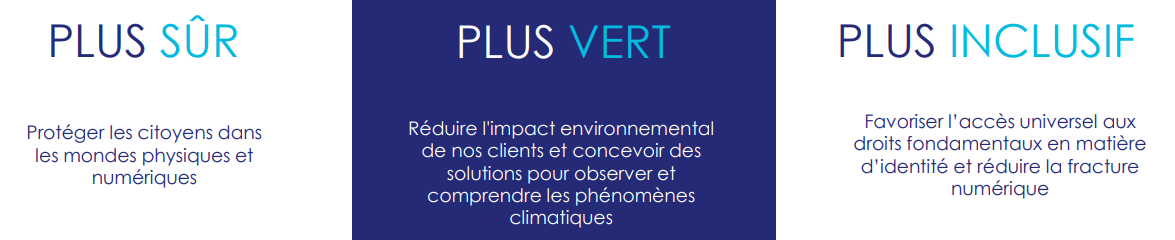
\includegraphics[width=\textwidth]{img/thales_mission.png}
	\caption{Axes majeurs du développement à Thales}
	\label{thalesmission}
\end{figure}

\noindent Au sein de Thales existent 7 GBUs : 
\begin{itemize}
	\item Avionics (AVS)
	\item Digital Identity \& Security (DIS) 
	\item Secure Communications \& Information Systems (SIX) 
	\item Defence Mission Systems (DMS)  
	\item Ground Transportation Systems (GTS)
	\item Land \& Air Systems (LAS)
	\item Thales Alenia Space (TAS)
\end{itemize}
Mon stage se déroulait au sein de Thales Services Numériques dans la \hyperref[GBU]{GBU} SIX.

\subsection{Thales Service Numérique (TSN)}

Thales Services Numériques (TSN), dirigé par Walter Cappilati, est l’ESN du groupe Thales et a pour mission d’assurer la performance, la résilience et la sécurité des systèmes d’information de ses clients. TSN compte plus de 4 300 collaborateurs et propose des solutions pour de nombreux marchés : défense, transport, finances, aéronautique... \\ 

TSN travail à 30\% pour le groupe et à 70\% chez des clients hors Thales. TSN s’est fixé les objectifs suivants :
\begin{itemize}
	\item Être une entreprise de services numériques faisant preuve d’une croissance rentable plus rapide que le marché, et être reconnue comme une référence dans ses secteurs clés.
	\item Accentuer l’innovation, la capacité à accompagner la transformation numérique des clients, la maîtrise du développement de solutions sur mesure, la gestion des systèmes d’information les pluscritiques et la cybersécurité.
	\item Être un partenaire de confiance au sein du groupe Thales et auprès des clients privés et publics les plus exigeants, leur garantir la maîtrise d’un bout à l’autre des technologies numériques, au service de leurs enjeux de sécurité et de performance économique et opérationnelle. \\
\end{itemize}

Au sein de TSN existent 4 directions d’excellence technique : la direction du conseil numérique sécurisé (DCNS), la direction de l’ingénierie logicielle (DIL), la direction de l’ingénierie IT outsourcing (DIO) et la direction technique (DT). Ma place était au sein de la direction technique, entouré d’architectes sécurité.

\subsection{Direction Technique (DT)}

La fonction première de la Direction Technique consiste à garantir l’alignement technique nécessaire pour répondre aux enjeux de compétitivité des solutions, de bonne exécution technique des projets et de l’approche globale de la cybersécurité sur le périmètre de Thales Services Numériques La direction technique assure ses fonctions centrées sur le développement et l’animation de l’expertise technique, du domaine de l’infrastructure à celui du développement d’applications logicielles, aussi bien dans les phases de construction que d’opération. Pour assurer ses responsabilités, la direction technique s’appuie sur :

\begin{itemize}
	\item Une politique technique qui concerne les méthodes, les technologies et les outils à utiliser sur les projets. Elle définit le cadre d’application. La direction technique est donc garante du maintien de la politique technique.
	\item Une direction de l’innovation qui se charge de développer la partie recherche et développement nommée « Self-Funding Research \& Development » (SFRD).
	\item Une filière expertise comptant plus de 300 personnes. Cette filière a pour objectif d’intervenir en support stratégique et technique pour des équipes projets. Elle est composée d’architectes et experts, de « Strategic Technical Authority » (STA), de « Project Design Authority » (PDA) et de « Design Authority » (DA).
	\item Une forte synergie avec les autres directions pour identifier les partenariats techniques afin d’assurer la pérennité des solutions déployées.
\end{itemize}

\subsection{Le positionnement du stage dans les traveaux de l'entreprise}

L’équipe de sécurité de la Direction technique de Thales Services Numérique a pour objectif de garantir des solutions de haute sécurité pour les systèmes fournis en interne ou en externe (qu’ils soient à destination d’administrations Françaises ou de grandes entreprises). Dans ce contexte, un thème d’importance capitale est la protection des données, et notamment la confidentialité et le respect de la vie privée (RGPD). \\

Sakeyna est une suite de composants développés par Thales Services Numériques pour fournir des solutions de chiffrement de données et de signature électronique. Ces composants permettent de « cacher » la complexité des mécanismes cryptographiques en fournissant des interfaces de haut niveau, qui peuvent être facilement intégrées sans nécessiter une expertise cryptographique (qui reste une compétence rare), et qui évite des erreurs que ce soit dans le choix des mécanismes ou dans leur utilisation et implémentation. \\

Sakeyna a été initialement développé en Java, mais mon Tuteur, Mahmoud Chilali, souhaite porter cette application en Rust au vu des performances et du futur prometteur de ce relativement nouveau langage. Ma mission sera donc d'expérimenter avec ce nouveau langage pour fournir des applications pouvant servir de preuve de fonctionnement et simplifier la migration de Sakeyna.

\section{Travaux réalisé}
\subsection{Chiffrement}
\subsubsection{AES}\label{AESsec}
\noindent\emph{Toutes les informations qui m'ont permis d'écrire cette sous sous section sont directement tirées de \cite{courslong}.}\\

Face au manque de standard de chiffrement, le \hyperref[NIST]{NIST} a lancé un concours en 1997 pour créer un nouveau standard: AES (Advanced Encryption Standard). \\
De là naît un nouvel algorithme inspiré de la proposition des cryptographes belge Joan Daemen et Vincent Rijmen. Il permet de chiffrer des blocs de 128 bits et existe sous trois variantes\footnote{à l'origine cet algorithme pouvait supporter des blocs de 128, 192 et 256 bits. Cette fonctionnalité n'a malheureusement pas été conservé par \hyperref[NIST]{NIST}. Cette fonction aurait permis à AES d'être post quantique.}:
\begin{table}[H]
\center
\begin{tabular}{|c|c|c|c|}
\hline
	\makecell{nom} & \makecell{taille de la clef \\ (bits)} & \makecell{taille des blocs \\ (bits)} & \makecell{nombre de rounds} \\ \hline\hline
	AES 128 & 128 & 128 & 10 \\ \hline
	AES 192 & 192 & 128 & 12 \\ \hline
	AES 256 & 256 & 128 & 14 \\ \hline
\end{tabular}
\caption{Variantes d'AES}
\label{AES-versions}
\end{table}

\noindent\emph{A partir de maintenant, pour fluidifier la lecture, AES 128 = AES)} \\ 

Le fonctionnement d'AES est relativement simple en principe. Il traite son entrée (un bloc de 128 bits) en appliquant une permutation \hyperref[permutPi]{$\Pi$} répétée plusieurs fois, à l'exception du dernier tour où une permutation légèrement différente, notée \hyperref[permutPiChap]{$\hat\Pi$}, est utilisée. La particularité de ces deux permutations, \hyperref[permutPi]{$\Pi$} et \hyperref[permutPiChap]{$\hat\Pi$}, réside dans leur inversibilité, ce qui signifie qu'il est possible de retrouver l'entrée d'origine en appliquant l'opération inverse. Cette propriété permet de déchiffrer le message en remontant étape par étape le processus d'AES. \\
En plus de ces permutations, le résultat de chacune est soumis à une opération \hyperref[XOR]{XOR}\footnote{L'avantage du \hyperref[XOR]{XOR} est qu'il est auto-inverse, c'est-à-dire $\hyperref[XOR]{\text{XOR}}^2 = \text{id}$, donc $\hyperref[XOR]{\text{XOR}}^{-1} = \hyperref[XOR]{\text{XOR}}$. Ainsi, il suffit de réappliquer le \hyperref[XOR]{XOR} pour remonter le processus d'AES} avec une clé $k_i$ , où $i$ correspond au numéro du round\footnote{Un round est le passage dans une permutation}. Ces clés sont calculées à partir d'une unique clé secrète de 128 bits (voir \ref{clefki}).

\begin{figure}[h]
\centering
\begin{tikzpicture}[scale=.8]
	% textes
	\node[draw, rectangle, align=center] (input) at (0.2,0) {Entrée};

	\node[draw, scale=1.5, rectangle, align=center] (round1) at (3,0) {$\hyperref[permutPi]{\Pi}$};
\node[below, scale=0.75] at (round1.south) {round 1};
	\node[align=center] (dots) at (5.5,0) {$\dots$};
	\node[draw, scale=1.5, rectangle, align=center] (round9) at (8,0) {$\hyperref[permutPi]{\Pi}$};
	\node[below, scale=0.75] at (round9.south) {round 9};
	\node[draw, scale=1.5, rectangle, align=center] (round10) at (10.4,0) {$\hyperref[permutPiChap]{\hat\Pi}$};
	\node[below, scale=0.75] at (round10.south) {round 10};
	
	\node[draw, rectangle, align=center] (output) at (13.2,0) {Sortie};

	% XOR
	\node[scale=1.5, align=center] (xor1) at (1.8,0) {$\hyperref[XOR]{\oplus}$};
	\node[scale=0.75] at (xor1.north) {$k_0$};
	\node[scale=1.5, align=center] (xor2) at (4.2,0) {$\hyperref[XOR]{\oplus}$};
	\node[scale=0.75] at (xor2.north) {$k_1$};
	\node[scale=1.5, align=center] (xor3) at (6.8,0) {$\hyperref[XOR]{\oplus}$};
	\node[scale=0.75] at (xor3.north) {$k_7$};
	\node[scale=1.5, align=center] (xor4) at (9.2,0) {$\hyperref[XOR]{\oplus}$};
	\node[scale=0.75] at (xor4.north) {$k_8$};
	\node[scale=1.5, align=center] (xor5) at (11.6,0) {$\hyperref[XOR]{\oplus}$};
	\node[scale=0.75] at (xor5.north) {$k_9$};

	% lignes
	\draw (input.east) -- (round1.west);
	\draw (round1.east) -- (dots.west);
	\draw (dots.east) -- (round9.west);
	\draw (round9.east) -- (round10.west);
	\draw (round10.east) -- (output.west);
\end{tikzpicture}
\caption{fonctionnement d'AES}
\label{AES_fonctionnement}
\end{figure}

\paragraph{Permutation $\Pi$}\label{permutPi}
Cette permutation ne dépend pas des paramètres de l'algorithme et peut donc être précalculé\footnote{Cela permet une exécution très rapide}. Elle se décompose en trois sous-permutations (toutes inversibles): $\hyperref[subbytes]{\mathtt{SubBytes}}$, $\hyperref[shiftrows]{\mathtt{ShiftRows}}$ et $\hyperref[mixcolumns]{\mathtt{MixColumns}}$. Pour plus facilement comprendre ces 3 sous-permutations, il faut s'imaginer qu'un bloc de 128 bits\footnote{i.e 4 \hyperref[byte]{bytes}} est une matrice $4\times4$ où chaques cellules contient un \hyperref[byte]{byte}

\begin{figure}[h]
\centering
\begin{tikzpicture}
	% entrée
	\node[align=center] (s) at (0,0) {$s_0|s_1|\dots|s_{15}$};
	
	% matrice
   	\foreach \y in {-1,0,1,2} {
        	\foreach \x in {2,3,4,5} {
            	\draw (\x, -\y) rectangle (\x+1, -\y+1);
            
            	\pgfmathtruncatemacro{\number}{(\y+1)*4 + \x -2}
		\node at (\x + 0.5, -\y + 0.5){$s_{\number}$};
        }

	% fleche
	\draw[->] (s.east) -- (1.8,0);
    }
\end{tikzpicture}
\caption{Réorganisation d'un bloc de 128 bits}
\label{reorg_entre}
\end{figure}

Une fois ce passage au format matriciel admis, on peut facilement expliquer les sous-permutations : 
\begin{enumerate}
	\item $\mathtt{SubBytes}\label{subbytes}$ \\
		On applique à chaque élément de la matrice une permutation $S: \{0,1\}^8 \rightarrow \{0,1\}^8$ (donc d'un \hyperref[byte]{byte} vers un autre).

		\begin{figure}[h]
		\centering
		\begin{tikzpicture}
			\foreach \y in {-1,0,1,2} {
			\foreach \x in {0,1,2,3} {
				\draw (\x, -\y) rectangle (\x+1, -\y+1);
			    
				\pgfmathtruncatemacro{\number}{(\y+1)*4 + \x }
				\node at (\x + 0.5, -\y + 0.5){$s_{\number}$};
			}}

			% matrice
			\foreach \y in {-1,0,1,2} {
			\foreach \x in {6,7,8,9} {
				\draw (\x, -\y) rectangle (\x+1, -\y+1);
			    
				\pgfmathtruncatemacro{\number}{(\y+1)*4 + \x-6}
				\node at (\x + 0.5, -\y + 0.5){$\tilde{s}_{\number}$};
			}}

			% fleche
			\draw[->] (4.5,0) -- (5.5,0) node[midway, above, scale=0.8] {$\mathtt{SubBytes}$};
		\end{tikzpicture}
		\caption{Effet de $\mathtt{SubBytes}$ sur un bloc, avec $\tilde{s} = S(s)$}
		\label{illu_subbyte}
		\end{figure}

		\begin{center}RAJOUTER DEF S\end{center}

	\item $\mathtt{ShiftRows}$\label{shiftrows} \\
		Cette sous-permutation va, pour chaque colonne de la matrice, déplacer de manière cyclique ses éléments de telle manière que la colonne $i$ subira le cycle $$\left(0 \quad (1+i)\%4 \quad (2+i)\%4 \quad (3+i)\%4\right)$$

		\begin{figure}[H]
		\centering
		\begin{tikzpicture}
			\foreach \y in {-1,0,1,2} {
			\foreach \x in {0,1,2,3} {

				\draw (\x, -\y) rectangle (\x+1, -\y+1);
			    
				\pgfmathtruncatemacro{\number}{(\y+1)*4 + \x }
				\node at (\x + 0.5, -\y + 0.5){$s_{\number}$};
			}}

			% matrice
			\foreach \y in {-1,0,1,2} {
			\foreach \x in {6,7,8,9} {	
				\pgfmathtruncatemacro{\n}{(\y+2)*10}

				\fill[black!\n] (\x, -\y) rectangle (\x+1, -\y+1);
			    
				\pgfmathtruncatemacro{\number}{(\y+1)*4+\x-6}
				\pgfmathtruncatemacro{\nnumber}{\number+\y+1}
				\pgfmathtruncatemacro{\result}{
					mod(\nnumber, 4) + 4*(\y+1)
				}
				\node at (\x + 0.5, -\y + 0.5){$s_{\result}$};
			}}

			% fleche
			\draw[->] (4.5,0) -- (5.5,0) node[midway, above, scale=0.8] {$\mathtt{ShiftRows}$};
		\end{tikzpicture}
		\caption{Effet de $\mathtt{ShiftRows}$ sur un bloc}
		\label{illu_shiftrows}
		\end{figure}

	\item $\mathtt{MixColumns}$\label{mixcolumns} \\
		Pour cette permutation, on calcule dans \hyperref[GF]{$GF$}$\left(2^8\right)$\footnote{muni du polynôme irréductible $x^8 + x^4 + x^3 + x + 1$ ie $100011011$} le produit matriciel (à gauche) de notre bloc par:
		
		$$
		\begin{pmatrix}
			2 & 3 & 1 & 1 \\
			1 & 2 & 3 & 1 \\
			1 & 1 & 2 & 3 \\
			3 & 1 & 1 & 2 \\
		\end{pmatrix}
		$$
		
		\noindent avec les éléments de cette matrice à comprendre comme des éléments de \hyperref[GF]{$GF$}$\left(2^8\right)$. \\
\end{enumerate}

\noindent Donc, en résumé : 
$$
\begin{pmatrix}
	s_{0} & s_{1} & s_{2} & s_{3} \\
	s_{4} & s_{5} & s_{6} & s_{7} \\
	s_{8} & s_{9} & s_{10} & s_{11} \\
	s_{12} & s_{13} & s_{14} & s_{15} \\
\end{pmatrix}
\overset{\Pi}{\rightarrow}
\begin{pmatrix}
	2 & 3 & 1 & 1 \\
	1 & 2 & 3 & 1 \\
	1 & 1 & 2 & 3 \\
	3 & 1 & 1 & 2 \\
\end{pmatrix}
\times
\begin{pmatrix}
	\tilde{s}_0 & \tilde{s}_1 & \tilde{s}_2 & \tilde{s}_3 \\
	\tilde{s}_5 & \tilde{s}_6 & \tilde{s}_7 & \tilde{s}_4 \\
	\tilde{s}_{10} & \tilde{s}_{11} & \tilde{s}_8 & \tilde{s}_9 \\
	\tilde{s}_{15} & \tilde{s}_{12} & \tilde{s}_{13} & \tilde{s}_{14} \\
\end{pmatrix}
$$

\paragraph{Permutation $\hat{\Pi}$}\label{permutPiChap}
Généralement, on préfère utiliser $\hat{\Pi}$ au lieu de \hyperref[permutPi]{$\Pi$}  au dernier round pour avoir un algorithme de déchiffrement quasiment identique que celui de chiffrement. Avec $\hat{\Pi}$ définie telle que\footnote{C'est exactement $\Pi$ mais sans la permutation $\mathtt{MixColumns}$} :
$$
\begin{pmatrix}
	s_{0} & s_{1} & s_{2} & s_{3} \\
	s_{4} & s_{5} & s_{6} & s_{7} \\
	s_{8} & s_{9} & s_{10} & s_{11} \\
	s_{12} & s_{13} & s_{14} & s_{15} \\
\end{pmatrix}
\overset{\hat{\Pi}}{\rightarrow}
\begin{pmatrix}
	\tilde{s}_0 & \tilde{s}_1 & \tilde{s}_2 & \tilde{s}_3 \\
	\tilde{s}_5 & \tilde{s}_6 & \tilde{s}_7 & \tilde{s}_4 \\
	\tilde{s}_{10} & \tilde{s}_{11} & \tilde{s}_8 & \tilde{s}_9 \\
	\tilde{s}_{15} & \tilde{s}_{12} & \tilde{s}_{13} & \tilde{s}_{14} \\
\end{pmatrix}
$$
 
\paragraph{Création des clefs $k_i$}\label{clefki}
À partir d'une clef secrète $k$ (de 128 bits) il faut créer une série de clefs $k_0\dots k_{10}$.
Pour cela on sépare cette clef en 4 mots de 32 bits (4 \hyperref[byte]{byte}) chacun.

\begin{figure}[h]
\centering
\begin{tikzpicture}
	\node[align=center] (k) at (0,0) {$10110\dots0110$};
	\draw[thick] (-1.5,-0.5) -- (1.5,-0.5) node[midway, below, scale=0.8] {128 bits};
	
	\draw[->] (1.8,0) -- (2.5,0);
	
	\foreach \x in {3,4,5,6} {
		\pgfmathtruncatemacro{\n}{\x-3}
		\draw (\x, -0.5) rectangle (\x+1, 0.5);
		\node[align=center]  at (\x+0.5, 0) {$\omega_{\n}$};
	}
\end{tikzpicture}
\caption{réorganisation des clefs en suite de mots de 32 bits}
\label{illu_clef}
\end{figure}
\noindent On pose la première clef $k_0 = k = \fbox{$\omega_{0,0}|\omega_{0,1}|\omega_{0,2}|\omega_{0,3}$}$. Ensuite, on calcule $k_i = \fbox{$\omega_{i,0}|\omega_{i,1}|\omega_{i,2}|\omega_{i,3}$}$ une fonction de $k_{i-1}$ avec :

$$
\forall i \in \{1,2,3\} \quad 
\begin{cases}
	\omega_{i,0} &= \omega_{i-1,0} \oplus g_i(\omega_{i-1,3}) \\
	\omega_{i,j} &= \omega_{i-1,j} \oplus \omega_{i,j-1} \quad \forall j \in \{1,2,3\} 
\end{cases}
$$

\noindent Et $g: \{0,1\}^{32} \rightarrow \{0,1\}^{32}$ une fonction tirée des standards d'AES (voir \cite{aesnist}).


\subsubsection{AES CBC}\label{sectioncbc}
\noindent\emph{Toutes les informations qui m'ont permis d'écrire cette sous-section sont directement tirées de \cite{courscourt}.}\\

À lui seul, AES ne permet de chiffrer que des blocs de 128 bits. On pourrait se dire qu'il suffit d'appliquer AES sur l'ensemble des blocs (ça correspond à l'utilisation d'AES en mode ECB). 

\begin{figure}[h]
\centering
\begin{tikzpicture}
	% message clair
	\foreach \x in {0,2} {
		\pgfmathtruncatemacro{\n}{(\x)/2+1}
		\draw (\x, 0) rectangle (\x+2, 0.5);
		\node[align=center]  at (\x+1, 0.25) {$m_{\n}$};
	}
	\node[align=center]  at (5, 0.25) {$\dots$};

	% message caché
	\foreach \x in {0,2} {
		\pgfmathtruncatemacro{\n}{(\x)/2+1}
		\draw (\x, -2.5) rectangle (\x+2, -2);
		\node[align=center]  at (\x+1, -2.25) {$c_{\n}$};
	}
	\node[align=center]  at (5, -2.25) {$\dots$};
	
	\node[draw, rectangle, align=center] (e1) at (1,-1) {$\text{AES}_k$};
	\node[draw, rectangle, align=center] (e2) at (3,-1) {$\text{AES}_k$};

	\draw[line width = 0.6mm] (1,0) -- (e1.north);
	\draw[->, line width = 0.6mm] (e1.south) -- (1, -2);
	
	\draw[line width = 0.6mm] (3,0) -- (e2.north);
	\draw[->, line width = 0.6mm] (e2.south) -- (3, -2);
\end{tikzpicture}
\caption{Fonctionnement d'AES ECB, avec $\text{AES}_k$ le chiffrement d'un bloc par AES avec la clef secrète $k$}
\label{ilu_ECB}
\end{figure}

Mais, si on utilise la même clef sur plusieurs blocs, le chiffré devient très facile à déchiffrer. Il faudrait donc autant de clefs que de blocs pour assurer un chiffrement sécurisé. Cela doublerait la taille du message après le chiffrement, ce qui n'est pas du tout pratique.  Il faut donc trouver une autre manière d'utiliser AES de manière sécurisée sans pour autant se limiter à des données d'un bloc de 128 bits\footnote{dans la pratique, on ne chiffre quasiment jamais qu'un bloc, il faut donc un algorithme pour permettre à AES de chiffrer des données de plusieurs blocs}. Une solution proposée est d'utiliser AES en mode CBC (Cipher Block Chaining). \\

\begin{figure}[h]
\centering
\begin{subfigure}{\textwidth}
\centering
\begin{tikzpicture}
	% message clair
	\foreach \x in {0,2} {
		\pgfmathtruncatemacro{\n}{(\x)/2+1}
		\draw (\x, 0) rectangle (\x+2, 0.5);
		\node[align=center]  at (\x+1, 0.25) {$m_{\n}$};
	}
	\node[align=center]  at (5, 0.25) {$\dots$};

	% message caché
	\draw (-2,-3) rectangle (0,-2.5);
	\node[align=center]  at (-1, -2.75) {IV};
	\foreach \x in {0,2} {
		\pgfmathtruncatemacro{\n}{(\x)/2+1}
		\draw (\x, -3) rectangle (\x+2, -2.5);
		\node[align=center]  at (\x+1, -2.75) {$c_{\n}$};
	}
	\node[align=center]  at (5, -2.75) {$\dots$};
	
	\node[align=center, scale=1.5] (x1) at (0.5,-0.75) {$\hyperref[XOR]{\oplus}$};
	\node[draw, rectangle, align=center] (e1) at (0.5,-1.75) {$\text{AES}_k$};
	\node[align=center, scale=1.5] (x2) at (2.5,-0.75) {$\hyperref[XOR]{\oplus}$};
	\node[draw, rectangle, align=center] (e2) at (2.5,-1.75) {$\text{AES}_k$};


	\draw[->, line width = 0.6mm] (0.5,0) -- (x1.north);
	\draw[line width = 0.6mm] (x1.south) -- (e1.north);
	\draw[->, line width = 0.6mm] (e1.south) -- (0.5, -2.5);
	
	\draw[->, line width = 0.6mm] (2.5,0) -- (x2.north);
	\draw[line width = 0.6mm] (x2.south) -- (e2.north);
	\draw[->, line width = 0.6mm] (e2.south) -- (2.5, -2.5);
	

	\draw[->, line width = 0.6mm] (-0.5,-2.5) to[out=90, in=180] (x1.west);
	\draw[->, line width = 0.6mm] (1.5,-2.5) to[out=90, in=180] (x2.west);
	\node[align=center, scale=1.5, color=white] (xc) at (4.5,-0.75) {$\oplus$};
	\draw[->, line width = 0.6mm] (3.5,-2.5) to[out=90, in=180] (xc.west);

\end{tikzpicture}
\caption{Chiffrement}
\end{subfigure}

\begin{subfigure}{\textwidth}
\vspace{1cm}
\centering
\begin{tikzpicture}
	% message clair
	\draw (-2,0) rectangle (0,0.5);
	\node[align=center]  at (-1, 0.25) {IV};
	\foreach \x in {0,2} {
		\pgfmathtruncatemacro{\n}{(\x)/2+1}
		\draw (\x, 0) rectangle (\x+2, 0.5);
		\node[align=center]  at (\x+1, 0.25) {$c_{\n}$};
	}
	\node[align=center]  at (5, 0.25) {$\dots$};

	% message caché
	\foreach \x in {0,2} {
		\pgfmathtruncatemacro{\n}{(\x)/2+1}
		\draw (\x, -3) rectangle (\x+2, -2.5);
		\node[align=center]  at (\x+1, -2.75) {$m_{\n}$};
	}
	\node[align=center]  at (5, -2.75) {$\dots$};
	
	\node[draw, rectangle, align=center] (e1) at (0.5,-0.7) {$\text{AES}^{-1}_k$};
	\node[align=center, scale=1.5] (x1) at (0.5,-1.75) {$\hyperref[XOR]{\oplus}$};
	\node[draw, rectangle, align=center] (e2) at (2.5,-0.7) {$\text{AES}^{-1}_k$};
	\node[align=center, scale=1.5] (x2) at (2.5,-1.75) {$\hyperref[XOR]{\oplus}$};

	\draw[line width = 0.6mm] (0.5,0) -- (e1.north);
	\draw[->, line width = 0.6mm] (e1.south) -- (x1.north);
	\draw[->, line width = 0.6mm] (x1.south) -- (0.5, -2.5);
	
	\draw[line width = 0.6mm] (2.5,0) -- (e2.north);
	\draw[->, line width = 0.6mm] (e2.south) -- (x2.north);
	\draw[->, line width = 0.6mm] (x2.south) -- (2.5, -2.5);

	\draw[->, line width = 0.6mm] (-0.5,0) to[out=-90, in=180] (x1.west);
	\draw[->, line width = 0.6mm] (1.5,0) to[out=-90, in=180] (x2.west);
	\node[align=center, scale=1.5, color=white] (xc) at (4.5,-1.75) {$\oplus$};
	\draw[->, line width = 0.6mm] (3.5,0) to[out=-90, in=180] (xc.west);
\end{tikzpicture}
\caption{Déchiffrement}
\end{subfigure}
\caption{Fonctionnement d'AES CBC, avec $\text{AES}_k$ le chiffrement d'un bloc par AES avec la clef secrète $k$}
\label{ilu_cbc}
\end{figure}

Le premier bloc du chiffré est un Initialization Vector (IV), c'est un bloc choisi aléatoirement. \\
Ensuite, un deuxième point important est qu'il faut que la taille du message en clair soit exactement un multiple de 128 bits\footnote{c'est aussi vrai pour toutes les autres méthodes de chiffrement par bloc} La solution à ce problème\footnote{C'est un problème, car en pratique les données que l'on chiffre n'ont aucune raison d'avoir une taille multiple de 128} est de rajouter un padding. C'est-à-dire que l'on complète le message pour que sa taille soit exactement égale au prochain multiple de 128 bits\footnote{si le message est déjà un multiple de 128 bits on rajoute 128 bits de padding (i.e un bloc)}. 
En pratique, le padding peut prendre plein de forme différente, on peut compléter avec des $0$, des bits aléatoires, ect...\\ La seule règle importante est que le dernier \hyperref[byte]{byte} du bloc doit contenir le nombre de \hyperref[byte]{byte} de padding qui ont été rajoutés (entre 0 et 15)\footnote{Sinon on n'a aucun moyen de savoir ce qui faisait partie ou non du message original}. \\

Pour ma part, mon padding suivra la règle suivante : tous les \hyperref[byte]{byte}s du padding ont la même valeur (donc celle du dernier \hyperref[byte]{byte}).
Par exemple, s'il manque 3 \hyperref[byte]{byte}s à mon message pour être un multiple de 16 \hyperref[byte]{byte} (i.e 128 bites) alors, je rajoute à la fin du message $\fbox{02|02|02}$. Si c'est déjà un multiple de 16 \hyperref[byte]{byte} je rajoute à la fin\\ $\fbox{15|15|15|15|15|15|15|15|15|15|15|15|15|15|15|15}$.\\

J'ai aussi essayé d'implémenter un padding plus classique\footnote{On remplit de $0$ (par exemple pour un padding de 3 \hyperref[byte]{byte}s cela donne $\fbox{00|00|02}$)} mais j'ai du mal le faire, car ce type de padding me posais des problèmes dans \ref{padoracle} alors que la théorie m'assure que ça ne devrait pas être le cas. 

\paragraph{Mon implémentation}
Dans le cadre de ma mission, je dois implémenter AES CBC en RUST. 
J'ai choisi de ne pas réimplémenter AES, car j'avais du mal à implémenter des éléments relatif à $g$ (voir \ref{clefki}) mais aussi car une implémentation d'AES est très régulièrement inutilisable en pratique car trop facile à attaquer. Rien que des informations telles que la consommation électrique de l'ordinateur, le temps qu'il met à répondre ou encore le champ électromagnétique qu'il émet sont suffisantes pour casser une implémentation "normal"\footnote{La seule solution pour régler ce problème est d'utiliser directement les instructions du processeur}. \\

J'ai donc implémenté le mode CBC avec le padding énoncé à la fin de \ref{sectioncbc}. J'ai choisi pour simplifier la tâche de me restreindre à chiffrer des chaînes de caractères\footnote{C'est une des premières choses que j'ai faites dans mon stage. À l'époque, cette approche me semblait la plus intuitive et la plus simple. En fait, je me compliquais la vie sans le savoir. C'est bien plus simple de ne pas se préoccuper du type d'entrée et juste de tout convertir au format binaire}. De là est apparu un pseudo-problème, le type Char en RUST peut faire de 1 à 4 \hyperref[byte]{byte} (ce type est codé selon le standard \hyperref[utf]{UTF-8}). Mais, au déchiffrement, ne connaissant pas le nombre de \hyperref[byte]{byte} associé à chaque caractère, j'ai été dans l'obligation de faire comme si chaque caractère ne faisait qu'un \hyperref[byte]{byte}. Donc, si mon message n'est pas uniquement écrit avec des caractères \hyperref[ASCII]{ASCII}, j'aurais de la perte d'information. \\
Par exemple, si je chiffre et déchiffre le message : "Je vais à l'école" j'obtiendrai un message du type "Je vais \$£ l'\&ùcole" car les caractères "à" et "é" ne font pas partie du tableau \hyperref[ASCII]{ASCII} car ils sont codés sur plusieurs \hyperref[byte]{byte}s. 
J'ai choisi d'ignorer ce problème, étant donné qu'il n'est dû qu'au format de l'entrée.

\paragraph{Padding oracle attack}\label{padoracle}
Dans cette sous-sous-section, j'explique comment j'ai attaqué AES CBC et par extension tous les modes de chiffrement par bloc non authentifié (qui ne fournissent pas une preuve d'authenticité du chiffré). \\ 

L'attaque que j'ai menée repose sur un principe simple. Pour chaque algorithme de chiffrement qui utilisent un padding, l'attaquant trouvera toujours un moyen d'avoir un padding oracle\footnote{Avoir accès à un padding oracle, c'est pouvoir déduire du comportement du serveur si le padding du message que je lui demande de déchiffrer est correct (on peut par exemple déduire cette information du temps que met le serveur à nous répondre).} (pas encore de contre-exemples).
Je vais montrer ci-dessous qu'à partir du moment où on a accès à ce genre d'information, on peut déchiffrer le message.

\paragraph{Déchiffrer un bloc}
\noindent En reprenant la figure \ref{ilu_cbc} et en l'adaptant pour un bloc c on obtient la figure \ref{cbcdec1bloc}. 

\begin{figure}[h]
\centering
\begin{tikzpicture}
	\fill[red!20, opacity=0.5] (1.7,-0.1) rectangle (4.3,-3.35);
	% message clair
	\draw (0,0) rectangle (2,0.5);
	\node[align=center] at (1, 0.25) {IV};
	\draw (2,0) rectangle (4,0.5);
	\node[align=center] at (3,0.25) {c};

	% message caché
	\draw (2, -3) rectangle (4, -2.5);
	\node[align=center]  at (3, -2.75) {m};

	\node[draw, rectangle, align=center] (e2) at (3,-0.7) {$\text{AES}^{-1}_k$};
	\node[align=center, scale=1.5] (x2) at (3,-1.75) {$\hyperref[XOR]{\oplus}$};
	
	\draw[line width = 0.6mm] (3,0) -- (e2.north);
	\draw[->, line width = 0.6mm] (e2.south) -- (x2.north);
	\draw[->, line width = 0.6mm] (x2.south) -- (3, -2.5);

	\draw[->, line width = 0.6mm] (1,0) to[out=-90, in=180] (x2.west);

	\node[align=center] (pad_or) at (6,-2.75) {Padding Oracle};
	\draw[->, line width = 0.6mm] (4,-2.75) -- (pad_or.west);

\end{tikzpicture}
\caption{Déchiffrement d'un bloc (en rouge : ce qui ne nous est pas accessible)}
\label{cbcdec1bloc}
\end{figure}

\label{demodinpaddingracle}Le but de l'attaque est de trouver un IV tel que $m = \fbox{15|\dots|15}$ car si on y arrive alors, on a : 
$$ 
\text{IV} \oplus \text{AES}^{-1}_{k}\left(\text{c}\right) = \fbox{15|\dots|15} \quad \Rightarrow \quad \text{IV} \oplus \fbox{15|\dots|15} = \text{AES}^{-1}_{k}\left(\text{c}\right)
$$
On aura donc réussi à déchiffrer c! Pour arriver à trouver cet IV on procède de la manière suivante : \\

On pose IV = \fbox{$00$|$\dots$|$00$|b} avec b un \hyperref[byte]{byte} quelconque. On fait varier b (256 possibilités) jusqu'à obtenir une réponse positive du padding oracle. Une fois arrivé à cette étape il existe 2 situations dans lesquelles on peut se trouver :

\begin{enumerate}
	\item Dans le cas le plus courant, on aura m = \fbox{??|??|$\dots$|??|00}. C'est ce qu'on cherche!
	\item Mais il se peut aussi que l'avant-dernier \hyperref[byte]{byte} permette à plus d'un padding d'être correcte. En effet, si ce \hyperref[byte]{byte} vaut 01 alors, il existe un \hyperref[byte]{byte} b tel que l'IV produise un m = \fbox{??|??|$\dots$|??|01|01}.
\end{enumerate}
Ce deuxième cas est gênant, mais il est facile de vérifier dans quel cas on se trouve en modifiant l'avant-dernier \hyperref[byte]{byte} de l'IV.
En effet, si en modifiant l'avant-dernier \hyperref[byte]{byte} de l'IV, on a une réponse favorable du padding oracle, cela signifie qu'on est dans le premier cas, sinon on est dans le deuxième. 
\begin{align*}
	&\fbox{??|??|$\dots$|42|00} \rightarrow \text{padding valide}\\
	&\fbox{??|??|$\dots$|42|01} \rightarrow \text{padding invalide}
\end{align*}

Une fois à cette étape, on peut créer un IV qu'on appelle ZIV (zeroing IV). Cet IV permet de mettre à 0 les \hyperref[byte]{byte}s que l'on change dans m. Dans notre cas, on a directement IV = ZIV = $\text{ZIV}_{0}$\footnote{Car on a fait en sorte que notre IV produise un m du type \fbox{??|??|$\dots$|??|00}}\footnote{On note $\text{ZIV}_{\text{n}}$ l'IV qui impose que les n derniers bytes de m valent 00}. \\

\begin{figure}[h]
\centering
\begin{tikzpicture}
	\fill[red!20, opacity=0.5] (1,-0.1) rectangle (5,-3.35);
	% message clair
	\draw (0,0) rectangle (2,0.5);
	\node[align=center] at (1, 0.25) {$\text{ZIV}_{\text{n}}$};
	\draw (2,0) rectangle (4,0.5);
	\node[align=center] at (3,0.25) {c};

	% message caché
	\draw (1.2, -3) rectangle (1.8, -2.5) node[align=center] at (1.5, -2.75) {??};
	\draw (1.8, -3) rectangle (2.4, -2.5) node[align=center] at (2.1, -2.75) {$\dots$};
	\draw (2.4, -3) rectangle (3, -2.5) node[align=center] at (2.7, -2.75) {??};
	\draw (3, -3) rectangle (3.6, -2.5) node[align=center] at (3.3, -2.75) {00};
	\draw (3.6, -3) rectangle (4.2, -2.5) node[align=center] at (3.9, -2.75) {$\dots$};
	\draw (4.2, -3) rectangle (4.8, -2.5) node[align=center] at (4.5, -2.75) {00};

	\draw[thick] (2.9,-3.2) -- (4.9,-3.2) node[midway, below, scale=0.8] {n  \hyperref[byte]{byte}s zéroizé};

	\node[draw, rectangle, align=center] (e2) at (3,-0.7) {$\text{AES}^{-1}_k$};
	\node[align=center, scale=1.5] (x2) at (3,-1.75) {$\hyperref[XOR]{\oplus}$};
	
	\draw[line width = 0.6mm] (3,0) -- (e2.north);
	\draw[->, line width = 0.6mm] (e2.south) -- (x2.north);
	\draw[->, line width = 0.6mm] (x2.south) -- (3, -2.5);

	\draw[->, line width = 0.6mm] (1,0) to[out=-90, in=180] (x2.west);

	\node[align=center] (pad_or) at (7,-2.75) {Padding Oracle};
	\draw[->, line width = 0.6mm] (4.8,-2.75) -- (pad_or.west);

\end{tikzpicture}
\caption{Illustration de l'effet de $\text{ZIV}_{\text{n}}$ sur le message déchiffré par le serveur(en rouge : ce qui ne nous est pas accessible)}
\label{expliqueziv}
\end{figure}

\noindent On sait donc créer $\text{ZIV}_0$. Supposons que l'on soit capable créer $\text{ZIV}_n$, essayons de trouver $\text{ZIV}_{n+1}$. On pose 
$$\text{IV} = \text{ZIV}_n \hyperref[XOR]{\oplus} \fbox{00|$\dots$|00|b|n|$\dots$|n} \quad \text{avec n \hyperref[byte]{byte}s \fbox{n}}$$
 et b, un \hyperref[byte]{byte} quelconque (256 possibilités). Comme $0 \hyperref[XOR]{\oplus} x = x$\footnote{$0$ est l'élément neutre de \hyperref[XOR]{$\oplus$} dans $\mathbb{Z}/2\mathbb{Z}$}, alors on a 
$$\text{m} = \fbox{??|??|\dots|??|n|$\dots$|n} \quad \text{avec n \hyperref[byte]{byte}s \fbox{n}}$$
Comme à la première étape (celle qui permet de trouver $\text{ZIV}_0$), on fait varier b (256 possibilités) jusqu'à avoir une réponse positive du padding oracle. \\ En effectuant la même vérification qu'à la première étape, on est en mesure de trouver b tel que $\text{m} = \fbox{??|??|$\dots$|??|n|$\dots$|n|}$ avec cette fois-ci n+1 \hyperref[byte]{byte}s \fbox{n}. Alors
\begin{align*}
	m \hyperref[XOR]{\oplus} \fbox{00|$\dots$|00|n|$\dots$|n} &= \fbox{??|$\dots$|??|00|$\dots$|00} \\
	\Leftrightarrow	\underbrace{\fbox{??|??|\dots|??|n|$\dots$|n}}_{\text{avec n+1 \hyperref[byte]{byte}s \fbox{n}}} \hyperref[XOR]{\oplus} \underbrace{\fbox{00|$\dots$|00|n|$\dots$|n}}_{\text{avec n+1 \hyperref[byte]{byte}s \fbox{n}}} &= \underbrace{\fbox{??|$\dots$|??|00|$\dots$|00}}_{\text{avec n+1 \hyperref[byte]{byte}s \fbox{00}}}
\end{align*}
Donc 
\begin{align*}
	\text{IV} \hyperref[XOR]{\oplus} \overbrace{\fbox{00|$\dots$|00|n|$\dots$|n}}^{\text{avec n+1 \hyperref[byte]{byte}s \fbox{n}}} \hyperref[XOR]{\oplus} \text{AES}^{-1}_k\left(c\right) &= m \hyperref[XOR]{\oplus} \overbrace{\fbox{00|$\dots$|00|n|$\dots$|n}}^{\text{avec n+1 \hyperref[byte]{byte}s \fbox{n}}}\\
					&= \underbrace{\fbox{??|$\dots$|??|00|$\dots$|00}}_{\text{avec n+1 \hyperref[byte]{byte}s \fbox{00}}}\end{align*}
Et on cherche $\text{ZIV}_{n+1}$ tel que 
$$\text{ZIV}_{n+1} \hyperref[XOR]{\oplus} \text{AES}^{-1}_k\left(c\right) = \underbrace{\fbox{??|$\dots$|??|00|$\dots$|00}}_{\text{avec n+1 \hyperref[byte]{byte}s \fbox{00}}}$$
Donc par identification
\begin{align*}
	\text{ZIV}_{n+1} &= \text{IV} \hyperref[XOR]{\oplus} \fbox{00|$\dots$|00|n|$\dots$|n}\\
			 &= \text{ZIV}_n \hyperref[XOR]{\oplus} \underbrace{\fbox{00|$\dots$|00|b|n|$\dots$|n}}_{\text{avec n \hyperref[byte]{byte}s \fbox{n}}} \oplus \underbrace{\fbox{00|$\dots$|00|n|$\dots$|n}}_{\text{avec n+1 \hyperref[byte]{byte}s \fbox{n}}}
\end{align*}
D'où l'hérédité. On a donc montré par récurrence que $\forall n$\footnote{dans notre cas comme on a des blocs de 16 \hyperref[byte]{bytes}, $\forall n\in\llbracket0;~15\rrbracket$}, on peut trouver $\text{ZIV}_n$.\\
Or, on sait que (voir \ref{pad_ora_blo})
$$\text{AES}^{-1}\left(c\right) = \text{ZIV}_{15}$$
Donc, on a déchiffré le bloc c en trouvant $\text{ZIV}_{15}$ 
\begin{figure}[h]
\centering
\begin{tikzpicture}
	\fill[red!20, opacity=0.5] (1.7,-0.1) rectangle (4.3,-3.35);

	% message clair
	\draw (0,0) rectangle (2,0.5);
	\node[align=center, scale=0.8] at (1, 0.25) {$\text{AES}_k^{-1}(\text{c})$};
	\draw (2,0) rectangle (4,0.5);
	\node[align=center] at (3,0.25) {c};

	% message caché
	%\draw (2, -3) rectangle (4, -2.5);
	%\node[align=center]  at (3, -2.75) {$00|\dots|00$};
	\draw (2,-3) rectangle (2.66,-2.5) node[align=center] at (2.33,-2.75) {00};
	\draw (2.66,-3) rectangle (3.33,-2.5) node[align=center] at (3,-2.75) {$\dots$};
	\draw (3.33,-3) rectangle (4,-2.5) node[align=center] at (3.62,-2.75) {00};

	\node[draw, rectangle, align=center] (e2) at (3,-0.7) {$\text{AES}^{-1}_k$};
	\node[align=center, scale=1.5] (x2) at (3,-1.75) {$\hyperref[XOR]{\oplus}$};
	
	\draw[line width = 0.6mm] (3,0) -- (e2.north);
	\draw[->, line width = 0.6mm] (e2.south) -- (x2.north);
	\draw[->, line width = 0.6mm] (x2.south) -- (3, -2.5);

	\draw[->, line width = 0.6mm] (1,0) to[out=-90, in=180] (x2.west);

\end{tikzpicture}
\caption{Déchiffrement d'un bloc, (en rouge : ce qui ne nous est pas accessible)}
\label{pad_ora_blo}
\end{figure}

\paragraph{Généralisation à n blocs}
On rappelle le schéma de déchiffrement d'AES CBC sur la figure \ref{dechif_cbc}. On remarque alors qu'on peut très facilement généraliser à n blocs ce que l'on a fait pour un bloc, car pour trouver $c_i$ il suffit de faire comme si $c_{i-1}$ est l'IV et on remonte comme ça jusqu'à avoir trouvé tous les $c_i$.  

\begin{figure}[h]
\centering
\begin{tikzpicture}
	\fill[red!20, opacity=0.5] (-0.7,-0.1) rectangle (5.5,-3.35);

	% message clair
	\draw (-2,0) rectangle (0,0.5);
	\node[align=center]  at (-1, 0.25) {IV};
	\foreach \x in {0,2} {
		\pgfmathtruncatemacro{\n}{(\x)/2+1}
		\draw (\x, 0) rectangle (\x+2, 0.5);
		\node[align=center]  at (\x+1, 0.25) {$c_{\n}$};
	}
	\node[align=center]  at (5, 0.25) {$\dots$};

	% message caché
	\foreach \x in {0,2} {
		\pgfmathtruncatemacro{\n}{(\x)/2+1}
		\draw (\x-0.5, -3) rectangle (\x+1.5, -2.5);
		\node[align=center]  at (\x+0.5, -2.75) {$m_{\n}$};
	}
	\node[align=center]  at (4.5, -2.75) {$\dots$};
	
	\node[draw, rectangle, align=center] (e1) at (0.5,-0.7) {$\text{AES}^{-1}_k$};
	\node[align=center, scale=1.5] (x1) at (0.5,-1.75) {$\hyperref[XOR]{\oplus}$};
	\node[draw, rectangle, align=center] (e2) at (2.5,-0.7) {$\text{AES}^{-1}_k$};
	\node[align=center, scale=1.5] (x2) at (2.5,-1.75) {$\hyperref[XOR]{\oplus}$};

	\draw[line width = 0.6mm] (0.5,0) -- (e1.north);
	\draw[->, line width = 0.6mm] (e1.south) -- (x1.north);
	\draw[->, line width = 0.6mm] (x1.south) -- (0.5, -2.5);
	
	\draw[line width = 0.6mm] (2.5,0) -- (e2.north);
	\draw[->, line width = 0.6mm] (e2.south) -- (x2.north);
	\draw[->, line width = 0.6mm] (x2.south) -- (2.5, -2.5);

	\draw[->, line width = 0.6mm] (-0.5,0) to[out=-90, in=180] (x1.west);
	\draw[->, line width = 0.6mm] (1.5,0) to[out=-90, in=180] (x2.west);
	\node[align=center, scale=1.5, opacity=0] (xc) at (4.5,-1.75) {$\oplus$};
	\draw[->, line width = 0.6mm] (3.5,0) to[out=-90, in=180] (xc.west);
\end{tikzpicture}
\caption{Déchiffrement d'AES CBC avec en rouge ce qui ne nous est pas accessible}
\label{dechif_cbc}
\end{figure}

\subsubsection{AES GCM}
\noindent\emph{Toutes les informations qui m'ont permis d'écrire cette sous-section sont directement tirées de \cite{courscourt}.}\\


On s'est intéressé dans la sous-section précédente au mode CBC en montrant qu'AES CBC était facilement attaquable et donc pas fiable. On s'intéresse ici au mode GCM (Galois Counter Mode), le mode d'utilisation le plus courant d'AES. Comme pour AES CBC, AES GCM fait des opérations sur des blocs de 128 bits pour permettre de chiffrer de grands fichiers. Mais, à la différence d'AES CBC, AES GCM utilise un algorithme d'authentification en parallèle du chiffrement, ce qui permet d'assurer que le chiffré n'a pas été changé. Cette deuxième partie est essentielle, car il a été montré qu'un algorithme de chiffrement non authentifié est quasiment systématiquement attaquable.

\paragraph{CTR} \label{CTR}
Comme CBC, CTR (Counter) est un mode de manipulation des blocs qui permet de chiffrer des données avec des algorithmes de chiffrement par blocs (comme AES) tout en garantissant un certain niveau de sécurité. CTR, c'est GCM mais sans l'authentification. Il est assez similaire à CBC mais à comme gros avantage de ne pas obliger de rajouter un padding à la fin des données claires. Son fonctionnement est décrit sur la figure \ref{aesctr}. 

\begin{figure}[h]
\centering
\begin{tikzpicture}
	% message clair
	\foreach \x in {0,2} {
		\pgfmathtruncatemacro{\n}{(\x)/2+1}
		\draw (\x, 0) rectangle (\x+2, 0.5);
		\node[align=center]  at (\x+1, 0.25) {$m_{\n}$};
	}
	\node[align=center]  at (5, 0.25) {$\dots$};

	% message caché
	\draw (-2,-3.25) rectangle (0,-2.75);
	\node[align=center]  at (-1, -3) {IV};
	\foreach \x in {0,2} {
		\pgfmathtruncatemacro{\n}{(\x)/2+1}
		\draw (\x, -3.25) rectangle (\x+2, -2.75);
		\node[align=center]  at (\x+1, -3) {$c_{\n}$};
	}
	\node[align=center]  at (5, -3) {$\dots$};
	
	\node[draw, rectangle, align=center, scale = 0.75] (x1) at (1,-1.25) {$\text{AES}_k$};
	\node[align=center, scale=1.5] (e1) at (1,-2) {$\oplus$};
	\node[draw, rectangle, align=center, scale = 0.75] (x2) at (3,-1.25) {$\text{AES}_k$};
	\node[align=center, scale=1.5] (e2) at (3,-2) {$\oplus$};

	\draw[line width = 0.6mm] (x1.south) -- (e1.north);
	\draw[->, line width = 0.6mm] (e1.south) -- (1, -2.75);
	
	\draw[line width = 0.6mm] (x2.south) -- (e2.north);
	\draw[->, line width = 0.6mm] (e2.south) -- (3, -2.75);
	
	\node[align=center, scale = 0.75] (c1) at (1.5,-0.5) {$+1$};
	\node[align=center, scale = 0.75] (c2) at (3.5,-0.5) {$+1$};

	
	\draw[-, line width = 0.6mm] (-0.5,-2.75) -- (-0.5, -1);
	\draw[-, line width = 0.6mm] (-0,-0.5) -- (c1.west);
	\draw[-, line width = 0.6mm] (-0.5,-1) to[out=90, in=180] (0, -0.5);

	\draw[-, line width = 0.6mm] (c1.east) -- (c2.west);
	\draw[->, line width = 0.6mm] (c2.east) -- (4.5, -0.5);

	\draw[->, line width = 0.6mm] (0.5,-0.5) to[out=0, in=90] (x1.north);
	\draw[->, line width = 0.6mm] (2.5,-0.5) to[out=0, in=90] (x2.north);

	\draw[white, line width = 1mm] (0.1,-0.5) -- (0.3,-0.5);
	\draw[white, line width = 1mm] (2.1,-0.5) -- (2.3,-0.5);
	\draw[->, line width = 0.6mm] (0.25,0) to[out=270, in=180] (e1.west);
	\draw[->, line width = 0.6mm] (2.25,0) to[out=270, in=180] (e2.west);

\end{tikzpicture}
\caption{Fonctionnement d'AES CTR, avec $\text{AES}_k$ le chiffrement d'un bloc par AES avec la clef secrète $k$, \emph{Le +1 signifie qu'on incrémente de 1 l'IV généré aléatoirement.}
}
\label{aesctr}
\end{figure}
\paragraph{GMAC} \label{GMAC}

Pour obtenir GCM il faut rajouter une étape d'authentification à CTR. Elle est faite par un algorithme incrémental GMAC (Galois Message Authentification Code). Cet algorithme produit au cours du chiffrement des blocs un Tag qui résume de manière sécurisée toutes les informations sur la donnée à chiffrer. L'intérêt de cela est que chaque entrée produira un Tag unique. Donc, si quelqu'un a modifié le chiffré, alors il y aura une erreur lors du déchiffrement. Cela permet de garantir que la donnée que vous déchiffrez est bien celle que l'on souhaite récupérer.

\begin{figure}[h]
\centering
\begin{tikzpicture}

	% message caché
	\draw (-2,-3.25) rectangle (0,-2.75);
	\node[align=center]  at (-1, -3) {IV};
	\foreach \x in {0,2} {
		\pgfmathtruncatemacro{\n}{(\x)/2+1}
		\draw (\x, -3.25) rectangle (\x+2, -2.75);
		\node[align=center]  at (\x+1, -3) {$c_{\n}$};
	}
	\node[align=center]  at (5, -3) {$\dots$};
	\node[align=center] (x) at (5, -3.9) {$\dots$};
	\node[align=center] (xx) at (5, -5.2) {$\dots$};

	\draw (6, -3.25) rectangle (8, -2.75);
	\node[align=center]  at (7, -3) {$c_{n}$};
	\draw (8, -3.25) rectangle (10, -2.75);
	\node[align=center]  at (9, -3) {Tag};

	\node[draw, rectangle, align=center, scale = 0.75] (add) at (-1,-3.9) {AAD};
	\node[draw, rectangle, align=center, scale = 0.75] (len) at (7,-4.8) {Taille du chiffré et de l'AAD};

	
	\node[align=center] (x0) at (0,-3.9) {$\times \text{H}$};
	\node[align=center] (x1) at (1,-3.9) {$\bigoplus$};
	\node[align=center] (x2) at (2,-3.9) {$\times \text{H}$};
	\node[align=center] (x3) at (3,-3.9) {$\bigoplus$};
	\node[align=center] (x4) at (4,-3.9) {$\times \text{H}$};
	\node[align=center] (x5) at (6,-3.9) {$\times \text{H}$};
	\node[align=center] (x6) at (7,-3.9) {$\bigoplus$};
	\node[align=center] (x7) at (8,-3.9) {$\times \text{H}$};
	\node[align=center] (x8) at (9,-3.9) {$\bigoplus$};
	\node[align=center] (x9) at (10,-3.9) {$\times \text{H}$};
	\node[align=center] (x10) at (11,-3.9) {$\bigoplus$};

	\draw[-, line width = 0.6mm] (add.east) -- (x0.west);
	\draw[->, line width = 0.6mm] (x0.east) -- (x1.west);
	\draw[-, line width = 0.6mm] (x1.east) -- (x2.west);
	\draw[->, line width = 0.6mm] (x2.east) -- (x3.west);
	\draw[-, line width = 0.6mm] (x3.east) -- (x4.west);
	\draw[-, line width = 0.6mm] (x4.east) -- (x.west);
	\draw[-, line width = 0.6mm] (x.east) -- (x5.west);
	\draw[->, line width = 0.6mm] (x5.east) -- (x6.west);
	\draw[-, line width = 0.6mm] (x6.east) -- (x7.west);
	\draw[->, line width = 0.6mm] (x7.east) -- (x8.west);
	\draw[-, line width = 0.6mm] (x8.east) -- (x9.west);
	\draw[->, line width = 0.6mm] (x9.east) -- (x10.west);

	\node[draw, rectangle, align=center, scale = 0.75] (aesiv) at (3,-5.2) {$\text{AES}_k$};

	\draw[-, line width = 0.6mm] (-1.7, -3.25) -- (-1.7, -4.7);
	\draw[-, line width = 0.6mm] (-1.7, -4.7) to[out=270, in=180] (-1.2,-5.2);
	\draw[->, line width = 0.6mm] (-1.2,-5.2) -- (aesiv.west);
	\draw[-, line width = 0.6mm] (aesiv.east) -- (xx.west);
	\draw[-, line width = 0.6mm] (xx.east) -- (10.5,-5.2);
	\draw[->, line width = 0.6mm] (10.5,-5.2) to[out=0, in=270] (x10.south);

	\draw[->, line width = 0.6mm] (1, -3.25) -- (x1.north);
	\draw[->, line width = 0.6mm] (3, -3.25) -- (x3.north);
	\draw[->, line width = 0.6mm] (7, -3.25) -- (x6.north);
	\draw[->, line width = 0.6mm] (len.east) to[out=0, in=270] (x8.south);
	\draw[-, line width = 0.6mm] (x10.north) -- (11,-3.4);
	\draw[-, line width = 0.6mm] (11,-3.4) to[out=90, in=0] (10.5,-3);
	\draw[->, line width = 0.6mm] (10.5,-3) -- (10, -3);

\end{tikzpicture}
\caption{Fonctionnement du GMAC, avec $\text{AES}_k$ le chiffrement d'un bloc par AES avec la clef secrète $k$, et $\times \text{H}$ la multiplication dans \hyperref[GF]{$GF$}$\left(2^{128}\right)$ par $\text{H} = \text{AES}_k\left({0}^{128}\right)$.}
\label{gmac}
\end{figure}

Dans la figure \ref{gmac}, une nouvelle entrée, appelée AAD (Additional Authenticated Data), est introduite. L'AAD est une donnée que l'on souhaite authentifier, mais pas chiffrer. Par exemple, imaginons que vous envoyez un mot de passe accompagné d'une adresse web. Vous voudriez chiffrer le mot de passe pour le protéger, tout en laissant l'adresse en clair. Cependant, si l'adresse n'est pas authentifiée, un attaquant pourrait la modifier, et vous ne le sauriez pas lors du déchiffrement. L'AAD permet de garantir que l'adresse n'a pas été altérée."

\paragraph{GCM}

GCM est la combinaison du mode CTR (voir \ref{CTR}) et de la création d'un Tag avec GMAC (voir \ref{GMAC}). Combiné à AES, cela nous donne l'algorithme de chiffrement authentifié le plus largement utilisé. Son fonctionnement est décrit sur la figure \ref{aesgcm}.

\begin{figure}[h]
\centering
\begin{tikzpicture}
	\fill[green!20, opacity=0.5] (-0.8,-0.2) rectangle (7.7,-2.55);
	\fill[red!20, opacity=0.5] (-2.2,-3.4) rectangle (11.5,-5.6);

	% message clair
	\foreach \x in {0,2} {
		\pgfmathtruncatemacro{\n}{(\x)/2+1}
		\draw (\x, 0) rectangle (\x+2, 0.5);
		\node[align=center]  at (\x+1, 0.25) {$m_{\n}$};
	}
	\node[align=center]  at (5, 0.25) {$\dots$};
	\node[align=center] (x) at (5, -0.5) {$\dots$};

	\draw (6, 0) rectangle (8, 0.5);
	\node[align=center]  at (7, 0.25) {$m_{n}$};
	
	\node[draw, rectangle, align=center, scale = 0.75] (x1) at (1,-1.25) {$\text{AES}_k$};
	\node[align=center] (e1) at (1,-2) {$\bigoplus$};
	\node[draw, rectangle, align=center, scale = 0.75] (x2) at (3,-1.25) {$\text{AES}_k$};
	\node[align=center] (e2) at (3,-2) {$\bigoplus$};
	\node[draw, rectangle, align=center, scale = 0.75] (x3) at (7,-1.25) {$\text{AES}_k$};
	\node[align=center] (e3) at (7,-2) {$\bigoplus$};



	\draw[line width = 0.6mm] (x1.south) -- (e1.north);
	\draw[->, line width = 0.6mm] (e1.south) -- (1, -2.75);
	
	\draw[line width = 0.6mm] (x2.south) -- (e2.north);
	\draw[->, line width = 0.6mm] (e2.south) -- (3, -2.75);

	\draw[line width = 0.6mm] (x3.south) -- (e3.north);
	\draw[->, line width = 0.6mm] (e3.south) -- (7, -2.75);
	
	\node[align=center, scale = 0.75] (c1) at (1.5,-0.5) {$+1$};
	\node[align=center, scale = 0.75] (c2) at (3.5,-0.5) {$+1$};
	
	\draw[-, line width = 0.6mm] (-0.5,-2.75) -- (-0.5, -1);
	\draw[-, line width = 0.6mm] (-0,-0.5) -- (c1.west);
	\draw[-, line width = 0.6mm] (-0.5,-1) to[out=90, in=180] (0, -0.5);

	\draw[-, line width = 0.6mm] (c1.east) -- (c2.west);
	\draw[-, line width = 0.6mm] (c2.east) -- (4.5, -0.5);

	\draw[->, line width = 0.6mm] (0.5,-0.5) to[out=0, in=90] (x1.north);
	\draw[->, line width = 0.6mm] (2.5,-0.5) to[out=0, in=90] (x2.north);
	\draw[-, line width = 0.6mm] (x.east) -- (6.5, -0.5);
	\draw[->, line width = 0.6mm] (6.5,-0.5) to[out=0, in=90] (x3.north);

	\draw[white, line width = 1mm] (0.1,-0.5) -- (0.3,-0.5);
	\draw[white, line width = 1mm] (2.1,-0.5) -- (2.3,-0.5);
	\draw[white, line width = 1mm] (6.1,-0.5) -- (6.3,-0.5);
	\draw[->, line width = 0.6mm] (0.25,0) to[out=270, in=180] (e1.west);
	\draw[->, line width = 0.6mm] (2.25,0) to[out=270, in=180] (e2.west);
	\draw[->, line width = 0.6mm] (6.25,0) to[out=270, in=180] (e3.west);


	% message caché
	\draw (-2,-3.25) rectangle (0,-2.75);
	\node[align=center]  at (-1, -3) {IV};
	\foreach \x in {0,2} {
		\pgfmathtruncatemacro{\n}{(\x)/2+1}
		\draw (\x, -3.25) rectangle (\x+2, -2.75);
		\node[align=center]  at (\x+1, -3) {$c_{\n}$};
	}
	\node[align=center]  at (5, -3) {$\dots$};
	\node[align=center] (x) at (5, -3.9) {$\dots$};
	\node[align=center] (xx) at (5, -5.2) {$\dots$};

	\draw (6, -3.25) rectangle (8, -2.75);
	\node[align=center]  at (7, -3) {$c_{n}$};
	\draw (8, -3.25) rectangle (10, -2.75);
	\node[align=center]  at (9, -3) {Tag};

	\node[draw, rectangle, align=center, scale = 0.75] (add) at (-1,-3.9) {AAD};
	\node[draw, rectangle, align=center, scale = 0.75] (len) at (7,-4.8) {Taille du chiffré et de l'AAD};

	
	\node[align=center] (x0) at (0,-3.9) {$\times \text{H}$};
	\node[align=center] (x1) at (1,-3.9) {$\bigoplus$};
	\node[align=center] (x2) at (2,-3.9) {$\times \text{H}$};
	\node[align=center] (x3) at (3,-3.9) {$\bigoplus$};
	\node[align=center] (x4) at (4,-3.9) {$\times \text{H}$};
	\node[align=center] (x5) at (6,-3.9) {$\times \text{H}$};
	\node[align=center] (x6) at (7,-3.9) {$\bigoplus$};
	\node[align=center] (x7) at (8,-3.9) {$\times \text{H}$};
	\node[align=center] (x8) at (9,-3.9) {$\bigoplus$};
	\node[align=center] (x9) at (10,-3.9) {$\times \text{H}$};
	\node[align=center] (x10) at (11,-3.9) {$\bigoplus$};

	\draw[-, line width = 0.6mm] (add.east) -- (x0.west);
	\draw[->, line width = 0.6mm] (x0.east) -- (x1.west);
	\draw[-, line width = 0.6mm] (x1.east) -- (x2.west);
	\draw[->, line width = 0.6mm] (x2.east) -- (x3.west);
	\draw[-, line width = 0.6mm] (x3.east) -- (x4.west);
	\draw[-, line width = 0.6mm] (x4.east) -- (x.west);
	\draw[-, line width = 0.6mm] (x.east) -- (x5.west);
	\draw[->, line width = 0.6mm] (x5.east) -- (x6.west);
	\draw[-, line width = 0.6mm] (x6.east) -- (x7.west);
	\draw[->, line width = 0.6mm] (x7.east) -- (x8.west);
	\draw[-, line width = 0.6mm] (x8.east) -- (x9.west);
	\draw[->, line width = 0.6mm] (x9.east) -- (x10.west);

	\node[draw, rectangle, align=center, scale = 0.75] (aesiv) at (3,-5.2) {$\text{AES}_k$};

	\draw[-, line width = 0.6mm] (-1.7, -3.25) -- (-1.7, -4.7);
	\draw[-, line width = 0.6mm] (-1.7, -4.7) to[out=270, in=180] (-1.2,-5.2);
	\draw[->, line width = 0.6mm] (-1.2,-5.2) -- (aesiv.west);
	\draw[-, line width = 0.6mm] (aesiv.east) -- (xx.west);
	\draw[-, line width = 0.6mm] (xx.east) -- (10.5,-5.2);
	\draw[->, line width = 0.6mm] (10.5,-5.2) to[out=0, in=270] (x10.south);

	\draw[->, line width = 0.6mm] (1, -3.25) -- (x1.north);
	\draw[->, line width = 0.6mm] (3, -3.25) -- (x3.north);
	\draw[->, line width = 0.6mm] (7, -3.25) -- (x6.north);
	\draw[->, line width = 0.6mm] (len.east) to[out=0, in=270] (x8.south);
	\draw[-, line width = 0.6mm] (x10.north) -- (11,-3.4);
	\draw[-, line width = 0.6mm] (11,-3.4) to[out=90, in=0] (10.5,-3);
	\draw[->, line width = 0.6mm] (10.5,-3) -- (10, -3);


\end{tikzpicture}
\caption{Fonctionnement d'AES GCM avec en vert CTR et en rouge GMAC}
\label{aesgcm}
\end{figure}


\noindent Pour résumer, AES GCM prend 4 entrées : 
\begin{enumerate}
	\item un nonce (ou IV) généré aléatoirement (que l'on choisit de mettre au début du chiffré pour réduire le nombre d'objets à stocker).
	\item une clef (de préférence générée aléatoirement)
	\item des données à chiffrer et authentifier 
	\item des données à authentifier (on peut aussi ne pas en fournir)
\end{enumerate}
\noindent et fournit 2 sorties :
\begin{enumerate}
	\item Le chiffré de la donnée à chiffrer
\item Le tag associé aux entrées (mis à la fin du chiffré)
\end{enumerate}

\subsubsection{Programme de chiffrement/déchiffrement}
\paragraph{Contexte}
Maintenant que j'ai pris connaissance des algorithmes pour chiffrer des données, je dois mettre en place une solution écrite en Rust qui permettra de chiffrer et de déchiffrer des fichiers. Cette solution devra permettre d'utiliser soit AES-GCM, soit ChaCha20-Poly1305 (un autre algorithme de chiffrement non détaillé précédemment).
Une optimisation que je pourrais envisager serait de proposer une version qui chiffrerait "au fil de l'eau", c'est-à-dire de manière progressive, bloc par bloc, à mesure que les données sont lues ou écrites. Cette méthode présente l'avantage de maintenir un coût constant en espace mémoire, car elle ne nécessite pas de charger l'intégralité du fichier en mémoire avant de le chiffrer. \\


Pour exécuter ce programme de chiffrement, il suffira d'utiliser les commandes suivantes\footnote{le programme de chiffrement s'appelle rucrypt et celui de déchiffrement rudecrypt} : 
\begin{center}
\begin{minipage}{.63\linewidth}
\begin{lstlisting}[language = shell]
rucrypt [options] < input > output
rudecrypt [options] < input > output
\end{lstlisting}
\end{minipage}
\end{center}
Les options permettront de choisir l'algorithme utilisé\footnote{Pour le moment, peuvent soit valoir "aes" pour AES-GCM, ou bien "cha" pour ChaCha20-Poly1305 ou encore "aes\_stream" pour la version au fil de l'eau d'AES-GCM}.

\paragraph{Mise en place}
Cette fois-ci, contrairement à Ed25519, je n'ai pas tout reprogrammé. J'ai décidé d'utiliser des crates de confiance, largement éprouvées. Pour les identifier, je me suis aidé d'un site qui référence toutes les solutions couramment utilisées pour la cryptographie en Rust \cite{bddrustcrypto}. Pour AES, j'utilise AES 256 (voir le tableau \ref{AES-versions}). Pour chaque algorithme, je dois donc générer, avant le chiffrement, une clé de 32 octets (256 bits) et un nonce (vecteur d'initialisation) de 12 octets (96 bits). Il est démontré que cacher le nonce n'a aucun intérêt en termes de sécurité. Je place donc le nonce en clair avant le texte chiffré. \\

On pourrait s'arrêter là, mais il est possible d'ajouter un niveau de sécurité supplémentaire. Actuellement, le chiffrement et le déchiffrement se font avec une seule clé (c'est-à-dire une clé symétrique). Le problème de cette symétrie est que toute personne ayant accès à cette clé peut lire le message en clair. Dans le cadre de ma mission, cela représente une potentielle faille. En effet, le but final de ce programme est de permettre la création de sauvegardes chiffrées de données. Il est donc préférable d'utiliser une clé asymétrique (une pour le chiffrement et une pour le déchiffrement). Dans ce cas de figure, tout le monde peut effectuer une sauvegarde de ses fichiers, mais seules les personnes autorisées pourront les récupérer. Cela permet de garder le contrôle sur les flux. Pour cette raison, je génère une clé privée et une clé publique RSA, avec laquelle je chiffre ma clé symétrique. Ainsi, seule la personne en possession de la clé privée pourra déchiffrer le document. Pour plus de simplicité, je place la clé symétrique chiffrée avant le nonce.


$$
\text{rucrypt(data)} \rightarrow \fbox{RSA(clef symétrique) | nonce | data chiffré}
$$
\subsection{HSM} \label{HSMsec}

Le but du cryptographe est de créer des problèmes faciles à résoudre quand on a la clefs, mais beaucoup trop longs à casser sinon. Donc, dans beaucoup de cas, trouver un moyen de récupérer cette clef est beaucoup plus raisonnable que de chercher une faille dans le cryptosystème. Il faut donc trouver un moyen sécurisé pour garder nos clefs, i.e, il faut un coffre-fort moderne. \\

Pour cela, il existe les HSM (Hardware Securty Module) qui sont des dispositifs physiques dédiés à la gestion, au stockage et à la protection des clefs cryptographiques. Ils sont conçus pour exécuter des opérations cryptographiques, telles que le chiffrement, le déchiffrement, la signature numérique et la gestion de clés, de manière sécurisée.


\begin{figure}[h]
	\centering
	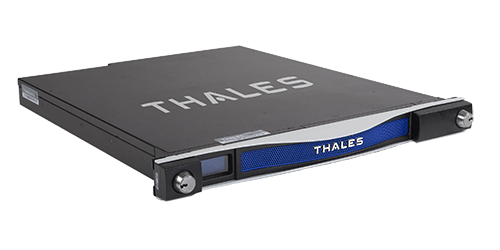
\includegraphics[width=.7\textwidth]{img/hsm.png}
	\caption{HSM de Thales}
	\label{hsmthales}
\end{figure}

Ici on ne n'intéressera pas réellement aux HSM mais plutôt aux SoftHSM, une implémentation logicielle d'un HSM. Ils permettent de développer des programmes, de faire des tests en amont d'une utilisation d'un HSM. \\

Dans un premier temps, j'ai dû me familiariser avec ce nouvel objet, puis, j'ai dû regarder les solutions en Rust qui nous permettent de communiquer avec des HSM, de les documenter et de les tester (via un SoftHSM). \\


Pour communiquer avec un SoftHSM j'ai dû me plonger dans la documentation du logiciel. Avant de pouvoir entamer des opérations cryptographiques, il faut créer un environnement dédié dans le SoftHSM. 
Pour le créer, la commande est la suivante :
\begin{center}
\begin{minipage}{\linewidth}
\begin{lstlisting}[language = shell]
sudo softhsm2-util --init-token --slot <slot-num> --token <token-label>
\end{lstlisting}
\end{minipage}
\end{center}
et pour le supprimer :
\begin{center}
\begin{minipage}{\linewidth}
\begin{lstlisting}[language = shell]
sudo softhsm2-util --delete-token --label <token-label>
\end{lstlisting}
\end{minipage}
\end{center}
Ici, il faut bien comprendre qu'un token est une émulation d'un HSM (on peut émuler plusieurs HSM sur un SoftHSM), le slot est un point d'entrée d'un HSM, il simule l'endroit ou l'on insère nos informations dans un HSM). \\
Après avoir initialisé mon softHSM, je peux communiquer avec lui en utilisant le standard pkcs11. C'est cette partie plus tard que je devrais programmer en Rust. Pour le moment, j'utilise OpenSSL, un logiciel qui me permet directement de communiquer avec le SoftHSM. Après avoir étudié la documentation, j'en ai tiré les informations suivantes : Pour créer une clef, je dois utiliser 
\begin{center}
\begin{minipage}{\linewidth}
\begin{lstlisting}[language = shell]
sudo pkcs11-tool --module /usr/lib/softhsm/libsofthsm2.so -l -p <usr-PIN> --keygen --key-type <enc-mech> --id <clef-id> --label <clef-label>
\end{lstlisting}
\end{minipage}
\end{center}
Avec <enc-mech> qui prend la forme AES:16, AES:32, ect. Pour la supprimer on utilise la commande : 
\begin{center}
\begin{minipage}{\linewidth}
\begin{lstlisting}[language = shell]
sudo pkcs11-tool --module /usr/lib/softhsm/libsofthsm2.so -l -p <usr-PIN> -b --type secrkey --id <clef-ID>
\end{lstlisting}
\end{minipage}
\end{center}
Maintenant qu'on a réussi à créer des clefs, on peut les utiliser pour chiffrer et déchiffrer des données. Pour le faire, il faut utiliser :
\begin{center}
\begin{minipage}{\linewidth}
\begin{lstlisting}[language = shell]
sudo pkcs11-tool --module /usr/lib/softhsm/libsofthsm2.so --login -p <usr-PIN> --encrypt --id <key-ID> -m AES-CBC-PAD --iv <iv-value> -i <input file> -o <output file>

sudo pkcs11-tool --module /usr/lib/softhsm/libsofthsm2.so --login -p <usr-PIN> --decrypt --id <key-ID> -m AES-CBC-PAD --iv <iv-value> -i <input file> -o <output file>
\end{lstlisting}
\end{minipage}
\end{center}
Pour la suite, j'utilise la crate cryptoki de Rust que j'ai trouvée grâce à \cite{bddrustcrypto}, ce qui me permet de garantir sa fiabilité.
La documentation de cette crate n'étant pas encore faite, j'ai créé un fichier tuto dans lequel je réalise toutes les opérations que je pourrais être amené à faire sur le SoftHSM, c'est-à-dire créer et supprimer des clés ainsi que chiffrer et déchiffrer des données. Pour y arriver, j'ai parcouru le code source de la documentation et je me suis aidé d'outils tels que ChatGPT. Après beaucoup d'essais, j'ai fini par obtenir un tutoriel fonctionnel.\\

La dernière étape consistait à vérifier que les résultats produits par mon programme correspondaient bien aux attentes. Pour cela, il est nécessaire de tester le programme avec des vecteurs de test. Chaque vecteur de test fournit une clé, un IV (Initialisation Vector), des données à chiffrer, le résultat chiffré attendu, et, si le programme le permet, des données à authentifier ainsi que le TAG correspondant. L'objectif de ces vecteurs est de comparer les sorties théoriques avec celles produites par notre algorithme. Pour que les tests soient validés, il faut que ces dernières soient identiques. \\

Pour faire ces tests, j'ai eu une grosse difficulté : je ne peux pas imposer la valeur d'une clef via mon programme (c'est une donnée protégée donc le softhsm me l'interdit). Pour contourner ce problème, je lance un script bash dans mon code Rust qui crée la clef avec OpenSSL. Ce script est le suivant : 
\begin{center}
\begin{minipage}{\linewidth}
\begin{lstlisting}[language = shell]
echo -n <key-value> > aes_key.txt
xxd -r -p aes_key.txt > aes_key.bin
sudo pkcs11-tool --module /usr/lib/softhsm/libsofthsm2.so -l -p <usr-PIN> --write-object
aes_key.bin --type secrkey --key-type <enc-mech> --id <clef-id> --label <clef-label>
\end{lstlisting}
\end{minipage}
\end{center}
Mon programme a passé tous les tests, et donc, grâce à mon tutoriel, je suis maintenant capable de remplacer OpenSSL par un programme "maison" en Rust.

\subsection{Signature}
Pour compléter mes connaissances en cryptographie, j'ai eu à implémenter deux algorithmes de signature. Comme pour le Tag dans AES GCM (voir \ref{GMAC}), une signature électronique permet d'authentifier une donnée et de garantir son intégrité. Mais, contrairement au Tag, elle peut aussi servir comme une preuve dans un contexte légal. Avec une signature numérique, l'expéditeur ne peut pas nier avoir signé la donnée. En effet, on verra plus tard que les algorithmes utilisés nécessitent des clefs asymétriques : une clef publique et une clef privée. Comme seul l'expéditeur connait la clef privée, il est le seul à pouvoir signer le document.

\subsubsection{RSA}
\paragraph{Génération des clefs}\label{keygenRSA}
\noindent Pour créer la clef publique et la clef privée, il faut :
\begin{enumerate}
	\item Poser $n = pq$ avec $p$ et $q$ deux nombres premiers
	\item Calcluler $\varphi(n)$ (l'indicatrice d'euler), le nombre d'éléments inversibles de $\mathbb{Z}/n\mathbb{Z}$ i.e $\varphi\left( n\right) = (p-1)(q-1)$
	\item Choisir $e$, un entier premier avec $\varphi(n)$
	\item Calculer $d = e^{-1}$ dans $\mathbb{Z}/\varphi(n)\mathbb{Z}$ (existe car $e \wedge \varphi(n) = 1$) 
\end{enumerate}
On a alors une clef privée = $(n, d)$ et une clef publique = $(n,e)$. Pour des raisons de sécurité, il faut choisir $n$ et $d$ grands (au moins 3072 bits) mais $e$ peut être petit. On remarque alors le grand défault de RSA :  les clefs sont extrêmement grande. C'est la principale raison pour laquelle on essaye d'éviter d'utiliser RSA quand il faut générer plusieurs clefs. Ce problème ne fera que devenir de plus en plus important avec le temps, car il faut constamment adapter la taille des clefs avec l'apparition des nouveaux composants.

\paragraph{Signer avec RSA}
Pour une donnée quelconque $m$ on calcule $h = \text{hash}(m)$ avec hash une fonction de hashage telle que 
$$
\forall m, \, \text{hash}(m) < n
$$ 
\emph{Si cette condition n'est pas vérifiée, rien ne garantit que la signature pourra être vérifiée.}
Enfin, pour calculer la signature $s$ associée à m, on chiffre h en calculant 
$$
s = h^d \, \lbrack n \rbrack
$$
On remarque bien qu'on utilise la clef privée pour créer la signature.

\paragraph{Vérifier l'intégrité des données}
N'importe qui en possession de la clef publique $(n, e)$ est en mesure de dire si le message $\tilde{m}$ qu'il a reçu avec la signature $s$ est authentique (i.e $\tilde{m} = m$). \\
Pour cela, il faut calculer $\tilde{h} = \text{hash}(\tilde{m})$ et déchiffrer la signature en calculant $s^e \, \lbrack n \rbrack$. Son message est authentique si et seulement si 
$$
\tilde{h} = s^e \, \lbrack n \rbrack
$$
Car $s^e = h^{ed} = h \lbrack n \rbrack$, donc $\tilde{h} = s^e \, \lbrack n \rbrack \Leftrightarrow \tilde{h} = h \lbrack n \rbrack$. Cette dernière égalité modulaire souligne bien l'importance de la condition sur le hash.

\subsubsection{Courbes elliptiques avec Ed25519}\label{courbeEd25519}
Nous avons vu qu'il était possible de faire de la signature numérique avec RSA, mais que ce cryptosystème n'a qu'un intérêt très limité à la vue de la taille gigantesque des clefs. Une alternative bien plus performante que RSA serait un cryptosystème s'appuyant sur les courbes elliptiques.
\paragraph{Courbe elliptique}
\noindent Pour un corps $K$, on peut définir une courbe elliptique par une équation de la forme 
$$
y^2 + a_1xy + a_3y = x^3 + a_2x^2 +a_4x + a_6
$$
avec $(a_1,\, \dots, a_6) \in K^6$. On sait que ces courbes sont symétriques par rapport à l'axe des abscisses (donc si $P$ est sur la courbe alors $-P$ aussi). \\

\begin{figure}[h]
	\centering
	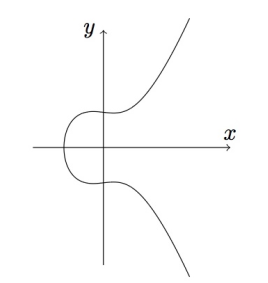
\includegraphics[width=.5\textwidth]{img/courbe1.png}
	\caption{Courbe $y^2 = x^3 - x + 9$ sur $\mathbb{R}$}
	\label{courbe1}
\end{figure}



\label{methodecorde}Un problème compliqué à résoudre sur ces courbes est de trouver les points rationnels de la courbe. Par contre, on sait qu'avec deux points $(U, V)$ rationnels tels que $U \neq -V$, on peut facilement en trouver deux autres. En effet, la droite qui passe par $U$ et $V$ coupera la courbe en un nouveau point $W$ rationnel (on a le quatrième point par symétrie).
De là, on définit l'addition sur une courbe elliptique par 
$$
U + V = - W
$$

\begin{figure}[h]
	\centering
	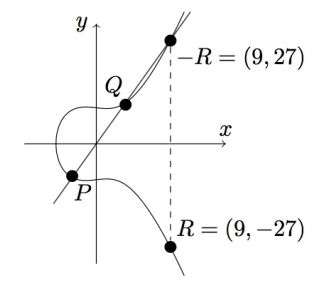
\includegraphics[width=.5\textwidth]{img/courbe1op.png}
	\caption{$P + Q$ sur $y^2 = x^3 - x + 9$ sur $\mathbb{R}$ avec $P = (-1-3)$ et $Q = (1,3)$}
	\label{courbe1op}
\end{figure}


\label{methodetangente}On peut étendre cette définition en partant d'un point rationnel $P$ de la courbe elliptique avec une ordonnée non nulle. Cette fois-ci, on prend sa tangente (on fait tendre $U$ et $V$ vers $P$, la droite qui passait par $U$ et $V$ tend bien vers la tangente passant par $P$). Alors cette tangente va bien couper la courbe en un deuxième point rationnel. Cette extention nous permet de définir $P+P$. \\

\noindent\emph{On appelle respectivement ces méthodes la méthode de la corde et de la tangente.}

\paragraph{Courbe elliptique sur un espace à dimension finie}
En cryptographie, on définit les courbes elliptiques sur des espaces à dimension finie de dimension $p$ : $\mathbb{Z}/p\mathbb{Z}$. Avec $p$ un premier supérieur à 3. \\
la courbe elliptique $(E)$ sur $ \mathbb{Z}/p\mathbb{Z}$ vérifiera 
$$
y^2 = x^3 + ax + b
$$
avec $(a,b) \in \left(\mathbb{Z}/p\mathbb{Z}\right)^2$ et $4a^3 + 27b^2 \neq 0$, cette condition permet d'éviter les singularités. \\

\begin{figure}[h]
	\centering
	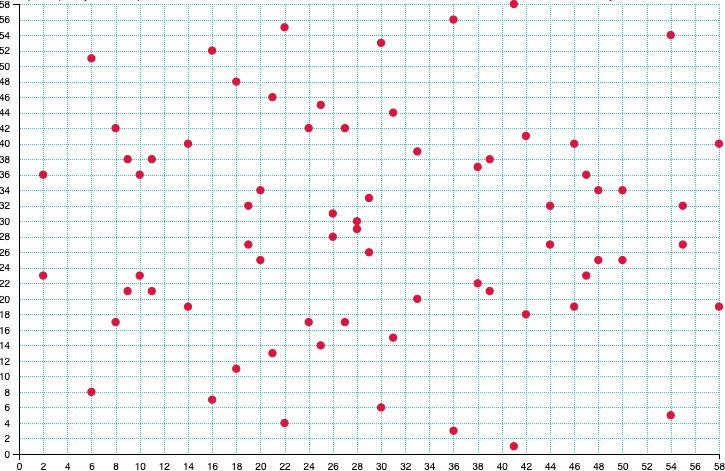
\includegraphics[width=.8\textwidth]{img/courbezpz.png}
	\caption{Courbe $y^2 = x^3 -6x + 2$ sur $ \mathbb{Z}/59\mathbb{Z}$}
	\label{courbezpz}
\end{figure}



\noindent On définit le groupe $\left(E\left( \mathbb{Z}/p\mathbb{Z} \right), +\right)$ par :
\begin{itemize}
	\item $E\left( \mathbb{Z}/p\mathbb{Z} \right)$ l'ensemble des points rationnels de la courbe $E$ définie sur $\mathbb{Z}/p\mathbb{Z}$
	\item $\mathcal{O}$ l'élément neutre pour l'addition définit comme le point de la courbe à l'infinit. Alors
		$$
		\forall P \in E\left( \mathbb{Z}/p\mathbb{Z} \right), \, P + \mathcal{O} = \mathcal{O}+P=P
		$$
	\item Posant $P = (x_1, y_1)$ et $Q = (x_2, y_2)$, on définit l'addition par ces trois règles pour calcluler $P+Q$ :
	\begin{enumerate}
		\item Si $x_1 \neq x_2$ on utilise la méthode de la corde (voir \ref{methodecorde})
		\item Sinon, si $P = Q$ on utilise la méthode de la tangente (voir \ref{methodetangente})
		\item Sinon ($P = -Q$) alors, on pose 
		$$
		P+Q = \mathcal{O}
		$$
	\end{enumerate}
	Voir \cite{courslong} si vous voulez voir les formules complètes.
\end{itemize}


\paragraph{Ed25519}\label{courbeed}

On s'intéresse maintenant à un cas particulier des courbes elliptiques (toujours sur $ \mathbb{Z}/p\mathbb{Z}$). On définit les courbes d'Edward comme des courbes elliptiques pouvant se mettre sous la forme 
$$
x^2 + y^2 = 1 + dx^2y^2
$$
avec $d \in \mathbb{Z}/p\mathbb{Z}$ et $d \neq 0,\, 1$. On peut alors définir + par
$
\forall (P,Q) = ((x_1,y_1),(x_2,y_2)) \in \left(E\left( \mathbb{Z}/p\mathbb{Z} \right)\right)^2
$
$$
P + Q = \left(\frac{x_1y_2+x_2y_1}{1+dx_1x_2y_1y_2},\, \frac{y_1y_2-x_1y_2}{1-dx_1x_2y_1y_2}\right), \quad \mathcal{O} = \left(0,1\right) 
$$
Cette simplicité d'implémentation permet de limiter certaines attaques. 

À partir de maintenant, on se concentre sur la courbe d'Edward avec $d = 3709570\\59346694393431380835087545651895421138798432190163887855330859402\\83555$ définit sur $ \mathbb{Z}/p\mathbb{Z}$ avec $p = 2^{255}-19$.


\paragraph{Génération des clefs}
\noindent Pour créer la clef publique et la clef privée, il faut :
\begin{enumerate}
	\item choisir un algorithme de hashage produisant un résultat sur 512 bits (généralement Sha512)
	\item créer une chaine $k$ de 256 bits (de préférence généré aléatoirement).
	\item calculer $h = hash(k)$ et puis $s$ à partir des 256 premiers bits de $h$ avec la convention "little endians".
	\item calculer $A = sB$ avec $B$\footnote{Pour des raisons de simplicité, calculatoire, on utilise une convention différente que celle présentée dans ici \ref{courbeed} mais elle est détaillée dans \cite{eddsa}} un point de Ed25519 donné dans \cite{eddsa}\\
\end{enumerate}

On a alors la clef privée $k$ et la clef publique $\text{compress}(A)$\footnote{compresse() est l'algorithme de compression de EdDSA. Dans notre cas, c'est une chaine de 256 bits. Les 255 premiers bits sont les 255 premiers bits de la coordonnée y du point en convention "little endians" (comme y<p, son bit de poids fort est tout le temps nul). Le dernier bit de la chaine vaut 1 si le point est négatif, 0 sinon}. On remarque bien que contrairement à RSA, EdDSA permet d'avoir des clefs bien plus petites (256 bits chacune).
\paragraph{Signer avec Ed25519}\label{signerEd25519}
Pour signer des données avec les courbes d'Edward on utilise l'algorithme EdDSA décrit plus précisément dans \cite{eddsa}.
Il y a des paramètres généraux propres à l'algorithme EdDSA sur Ed25519, mais je ne les présente pas. Pour les voir, je vous invite à lire la section 5.1 de \cite{eddsa}.\\

L'idée principale de cet algorithme est de générer à partir et du message et de la clef privée un point $R = rB$.
Pour calculer $r$, il faut calculer le hash modulo $L$\footnote{$L$ est une constante introduite dans \cite{eddsa} et vaut $2^{252}+2774231777737235353585193779088364\\8493$} des 256 derniers bits du hash de la clef privé $h = hash(k)$ concaténé à la donnée $m$ à signer.
$$
r = \text{hash}\left(h[32..64] \, \hyperref[concat]{\Vert} \, m\right) \, \lbrack L \rbrack
$$
Ensuite, on calcule $\tilde{h}$ tel que
$$
\tilde{h} = \text{hash}\left(\text{compress}(R) \, \hyperref[concat]{\Vert} \, \text{compress}(A) \, \hyperref[concat]{\Vert} \, m\right) \, \lbrack L \rbrack
$$
Enfin, notant $x = r+\tilde{h}s \lbrack L \rbrack$ en représentation "little endians" alors la signature est donnée par :
$$
\text{signature}_{\text{Ed25519}} = \text{compress}(R) \, \hyperref[concat]{\Vert} \, x
$$

On remarque que la signature fait 512 bits et a besoin de la clef privée et de la clef publique (dérive directement de la clef privée) pour la générer.

\paragraph{Vérifier l'intégrité des données}
N'importe qui en possession de la clef publique $A$ est en mesure de dire si le message $\tilde{m}$ qu'il a reçu avec la signature est authentique (i.e $\tilde{m} = m$). \\
Pour cela, il doit décompresser\footnote{Algorithme assez intuitif, mais avec des astuces de calcul détaillées dans \cite{eddsa}. Il consiste à récupérer la coordonnée $y$, à vérifier qu'il existe bien des points avec cette coordonée appartenant à la courbe, puis à choisir le bon point grâce au signe} le point $R$ en récupérant les 256 premiers bits de la signature. 
Ensuite, il faut récupérer l'entier $x$ écrit en convention "little endian" dans les 256 derniers bits de la signature et calculer. 
$$
\tilde{\tilde{h}} =  \text{hash}\left(\text{compress}(R) \, \hyperref[concat]{\Vert} \, \text{compress}(A) \, \hyperref[concat]{\Vert} \, \tilde{m}\right) \, \lbrack L \rbrack
$$
Enfin, le message sera authentique si et seulement si on a l'égalité dans le groupe $\left(E\left( \mathbb{Z}/p\mathbb{Z} \right), +\right)$
$$
xB = R + \tilde{\tilde{h}}A
$$
Car
\begin{align*}
	xB = R + \tilde{\tilde{h}}A \; &\Rightarrow \; rB + \tilde{h}sB = R+\tilde{\tilde{h}}A \\
							&\Rightarrow \; R + \tilde{h}A = R+\tilde{\tilde{h}}A \\
							&\Rightarrow \; \left(\tilde{h} - \tilde{\tilde{h}}\right)A = 0 \\
	\footnote{Argument géométrique}&\Rightarrow\; \tilde{h} = \tilde{\tilde{h}} \\
							&\Rightarrow \; m = \tilde{m}
\end{align*}
On remarque qu'on n'a bien besoin que de la clef publique $A$ pour vérifier la signature.

\subsubsection{Serveur signature}
Pour proposer ces services de signature, il est nécessaire de déployer un serveur qui recevra des données et renverra leurs signatures correspondantes. En pratique, c'est ainsi que les algorithmes de signature sont utilisés pour permettre aux entreprises de contrôler l'accès aux clés sensibles. De plus, j'ai intégré à ce serveur la possibilité de connexion à un HSM (cf \ref{HSMsec}) si nous en disposons, afin de renforcer la sécurité. Conformément à la demande de mon responsable, les données doivent être au format JSON et présenter le format suivant :

\begin{center}
\begin{minipage}{.51\linewidth}
\begin{lstlisting}[language = json]
{
 "id": "Vincent",
 "hash": "b16ed7d24b3ecb...",
 "methode": "sha512"
}
\end{lstlisting}
\end{minipage}
\end{center}
Afin de simplifier l'utilisation et de réduire le nombre de signatures nécessaires auprès du serveur (ce qui peut être lent avec un HSM), nous envoyons au serveur une liste ordonnée de données (l'ordre permet de garantir l'unicité de la signature pour chaque liste). Cela permet d'éviter la signature individuelle de chaque donnée tout en garantissant l'authenticité de l'ensemble des données de la liste.
\begin{center}
\begin{minipage}{.51\linewidth}
\begin{lstlisting}[language = json]
{
 "obj": [
  {
   "id": "Vincent",
   "hash": "b16ed7d24b3ecb...",
   "methode": "sha512"
  },
  {
   "id": "Alice",
   "hash": "6d201beeefb589...",
   "methode": "sha512"
  },
  {
   "id": "Bob",
   "hash": "cb872de2b8d250...",
   "methode": "sha512"
  }
 ]
}
\end{lstlisting}
\end{minipage}
\end{center}
En réalité, les données seront transmises à un client tiers, qui les hachera avant de les relayer au serveur. Cette approche offre une grande flexibilité, permettant ainsi à chaque partie prenante de configurer et d'utiliser son client de manière autonome.
\begin{figure}[h]
\centering
\begin{tikzpicture}
\node[align=center] (data) at (0,0) {data};	
\node[draw, rectangle, align=center] (client) at (3,0) {CLIENT};	
\node[draw, rectangle, align=center] (serveur) at (6,0) {SERVEUR};
\node[align=center] (signature) at (9,0) {signature};

\draw[->] (data.east) -- (client.west);
\draw[->] (client.east) -- node[midway, above] {hash} (serveur.west);
\draw[->] (serveur.east) to (signature.west);
\end{tikzpicture}
\caption{architecture du serveur signature}
\label{shema_serveur_signature}
\end{figure}

\subsection{Wireguard}
Maintenant, on veut créer à l'aide de Wireguard un flux chiffré entre plusieurs machines pour permettre à ces machines de communiquer de manière simple et sécurisée.
\subsubsection{Configuration}
Pour le serveur et les clients, il faut créer un fichier de configuration dans \\\verb+\ect\wireguard\wg0.conf+ (On n'est pas obligé de l'appeller \verb+wg0+). À l'intérieur, le fichier est séparé en au moins 2 sections :
\begin{itemize}
\item une qui commence par \verb+[Interface]+, elle contient les informations de la machine, comme la clef privée et l'adresse.
\item une autre (ou plus) qui commence par \verb+[Peer]+ et qui contient les informations des machines (comme la clef publique et les adresses autorisées) avec lesquelles on va communiquer. \\
\end{itemize}

Pour chaque machine, il faudra générer une paire de clefs. Pour cela, WireGuard nous fournit un outil. Il permet de créer une clé privée et de dériver la clé publique à partir de celle-là.

\begin{center}
\begin{minipage}{.6\linewidth}
\begin{lstlisting}[language = shell]
wg genkey > privatekey
wg pubkey < privatekey > publickey
\end{lstlisting}
\end{minipage}
\end{center}

\paragraph{Serveur}
Pour la configuration du serveur, il faut rajouter le port utilisé pour communiquer (typiquement 51820). Une configuration complète côté serveur pourra ressembler par exemple à

\begin{lstlisting}[language = shell]
[Interface]
PrivateKey = uKlFiRw6goZdHuPNeThISu7sGqr8JH3U+LrQ3VbaBXk= 
Address = 10.8.8.254/24
ListenPort = 51820

[Peer]
PublicKey = 4N2H/21U4kYpS5KZlQfjOjddlvs7bgr0Z3ZHHBqF8lU=
AllowedIPs = 10.8.8.1/32

[Peer] 
PublicKey = NIeEDlBPTJrM7389yaRKzXWJeAEicmrFm0zkfhnDVCo=  
AllowedIPs = 10.8.8.2/32
\end{lstlisting}
Chaque peer est un client avec lequel peut communiquer le serveur. Attention, il faut bien penser à activer l'IP forwarding du serveur pour lui permettre aux clients de communiquer entre eux (en pas uniquement au serveur). \\
Pour l'activer, il faut décommenter la ligne \verb+net.ipv4.ip_forward=1+ du fichier \\\verb+/etc/sysctl.conf+.

\paragraph{Clients}
La configuration d'un client est quasiment identique à celle d'un serveur, à la différence qu'il n'y a qu'un peer : le serveur. Elle ressemblera typiquement à 

\begin{lstlisting}[language = shell]
[Interface]
PrivateKey = uBl+tmfka8ukXcEV3vz5wtYinhZpLOEiAOe+gwhke28=
Address = 10.8.8.1

[Peer]
PublicKey = GigedMPFFe+r7SB4s48vnEnPREiAXX/TLB07hBuAGm4= 
Endpoint = 192.168.218.180:51820
AllowedIPs = 10.8.8.0/24
PersistentKeepalive = 25
\end{lstlisting}
La dernière ligne permet d'éviter d'avoir des problèmes, mais n'est pas obligatoire.
\subsubsection{Mise en place}
Pour activer la configuration, il suffit de lancer \verb+wg-quick up wg0+ et pour la désactiver \verb+wg-quick down wg0+. Maintenant, si on veut qu'elle s'active automatiquement quand la machine s'allume, il faut lancer \verb+sudo systemctl start wg-quick@wg0+(et \verb+sudo systemctl stop wg-quick@wg0+ pour que ça ne soit plus le cas). \\

Attention, pour l'instant, les clefs et les fichiers de configuration sont accessibles à tout le monde. Il faut veiller à supprimer les clefs (on n'en a plus besoin une fois qu'elles sont dans les fichiers de configuration) et à restreindre l'accès aux fichiers de configuration. 

\begin{center}
\begin{minipage}{.51\linewidth}
\begin{lstlisting}[language = shell]
sudo mkdir -p /etc/wireguard/
sudo chmod 700 /etc/wireguard
\end{lstlisting}
\end{minipage}
\end{center}

\subsection{Port knocking\protect\footnote{En réalité, je ne fais pas du Port knocking mais du SPA (Single Packet Authorization)  qui, à la différence du port knocking inclu de la cryptographie et est bien plus sécurisé}}
\subsubsection{Problème et solution}

Un des problèmes avec un canal comme on les utilise avec WireGuard est qu'ils sont ouverts en permanence. Ainsi, une personne qui a accès à un canal l'aura toujours. Une solution à ce problème peut être le port knocking. \\
En effet, le port knocking est une manière d'ouvrir temporairement un canal. Son fonctionnement est le suivant :

\begin{enumerate}
\item Le port de communication est fermé par défaut pour empêcher les accès non autorisés.
\item L'utilisateur envoie un paquet à un serveur \hyperref[UDP]{UDP} contenant une liste d'informations. Si le serveur arrive à identifier un utilisateur qui a le droit d'accéder au canal grâce à cette liste d'informations, alors il ouvre le port de communication.
\item Le port se referme automatiquement après un laps de temps défini.
\end{enumerate}
\subsubsection{Mon implémentation}
J'ai dû mettre en place le port knocking sur un canal WireGuard. Pour faire ça, j'ouvre un canal sans aucun Peer (personne ne peut communiquer sur ce canal). Le fichier de configuration de ce canal ressemble donc à ça 
\begin{lstlisting}[language = shell]
[Interface]
PrivateKey = 6GK6HC9adKr0OwGxU8jlidcTTh+A29clxBB+D1vUzXU= 
Address = 10.0.0.0/24
ListenPort = 51820
\end{lstlisting}
Ensuite, sur un serveur \hyperref[UDP]{UDP} je regarde si les paquets que je reçois contiennent une clef publique qui fait partie de la liste des clefs publiques autorisées (C'est comme ça que j'identifie un utilisateur). Si c'est le cas, j'édite le fichier de configuration pour rajouter le peer qui correspond à la clef publique et je mets à jour le canal. La configuration devient alors temporairement la suivante\footnote{Par contre, le fichier de configuration lui est toujours le même et si je redémarre le canal, alors on retourne à la configuration initiale.}
\begin{lstlisting}[language = shell]
[Interface]
PrivateKey = 6GK6HC9adKr0OwGxU8jlidcTTh+A29clxBB+D1vUzXU= 
Address = 10.0.0.0/24
ListenPort = 51820

[Peer]
PublicKey = 4N2H/21U4kYpS5KZlQfjOjddlvs7bgr0Z3ZHHBqF8lU=
AllowedIPs = 10.0.0.1/32
\end{lstlisting}
Ensuite, j'ai rajouté un compteur qui supprime automatiquement le nouveau peer au bout d'un moment. \\

\noindent Dans la pratique, pour envoyer un paquet au serveur, je dois rentrer 
\begin{center}
\begin{minipage}{.67\linewidth}
\begin{lstlisting}[language = shell]
nc -u -w 1 localhost 3000 < input.json
\end{lstlisting}
\end{minipage}
\end{center}
Avec un paquet au format json selon le standard suivant\footnote{Comme c'est un serveur UDP, on peut envoyer ce que l'on veut, mais on ne saura jamais s'il y a eu une erreur, c'est l'avantage de ce type de serveur.}
\begin{center}
\begin{minipage}{.51\linewidth}
\begin{lstlisting}[language = json]
{
  "allowed_ip": "10.0.0.0/24", 
  "key_pub": "GigedMPFFe+..."
}
\end{lstlisting}
\end{minipage}
\end{center}
Ensuite, le serveur regarde de temps en temps si l'utilisateur a toujours le droit d'utiliser le canal. Si ce n'est pas le cas, il le retire.

\subsection{Signal}
Dans l'idée de se débarrasser définitivement de RSA\footnote{On est capable de rendre RSA robuste à toute sorte d'attaque, mais cette robustesse à un prix énorme. Comme remarqué ici \ref{keygenRSA}. En effet, la taille des clefs ne cessant d'augmenter, son utilisation est de plus en plus contraignante.}, mon tuteur m'a chargé d'étudier et de recréer le protocole d'échange des clés de l'application Signal. Ce protocole a pour énorme avantage de permettre d'échanger les clefs sans avoir besoin au même moment des deux parties. On le qualifie de protocole d'échange asynchrone\footnote{En plus d'être asynchrone, ce protocole n'utilise pas RSA qui était à peu près la seule solution pour faire de l'asynchrone avant}.

\subsubsection{Extended Triple Diffie-Hellman (X3DH)}
\noindent\emph{Toutes les informations qui m'ont permis d'écrire cette sous-sous-section sont directement tirées de \cite{xtroisdh}.}\\

X3DH est un protocole d'échange de clef asynchrone qui met en jeu trois parties : Alice, Bob et un serveur. \\
Dans notre exemple, Alice (A) veut discuter avec Bob (B). Pour faire ça, ils doivent avoir un secret commun. Notre problème est que Bob n'est pas forcément là quand Alice veut générer ce secret. Pour tenter de résoudre ce problème, le serveur servira à Alice et à Bob d'intermédiaire.

\paragraph{Clefs}
Pour permettre cet échange, le serveur gardera pour chaque utilisateur un lot de clefs publiques\footnote{Des clefs pour courbes elliptiques comme Ed25519 \ref{courbeEd25519}}\footnote{les clefs secrètes correspondantes sont gardées sur la machine de l'utilisateur}. 
Pour l'utilisateur X (dans notre cas X = A (resp B) pour Alice (resp Bob))
\begin{itemize}
	\item $\text{IK}_{\text{X, pub}}$ la clef d'identité de X. Cette clef a une longue durée de vie (n'a pas besoin d'être changée souvent)
	\item $\text{EK}_{\text{X, pub}}$ une clef éphémère que X régénérée à chaque fois qu'il utilise X3DH.
	\item $\text{SPK}_{\text{X, pub}}$ une clef signée (avec $\text{IK}_{\text{X, priv}}$) qui peut changer de temps en temps. La signature est aussi sur le serveur. Cette clef est surtout importante dans \ref{doubleratchet}. 
	\item $\text{OPK}_{\text{X, pub}}$ une clef à utilisation unique. Dans la pratique, X3DH n'a pas réellement besoin d'OPK mais cela rajoute une couche de sécurité. Chaque utilisateur envoie au serveur une grande liste d'OPK la renouvelle assez souvent.
\end{itemize}
À tout moment, n'importe qui peut demander au serveur de lui donner ce lot de clefs.\\

Pour notre exemple (où Alice commence l'échange), on utilisera les clefs $\text{IK}_{\text{A}}$, $\text{EK}_{\text{A}}$, $\text{IK}_{\text{B}}$, $\text{SPK}_{\text{B}}$ et $\text{OPK}_{\text{B}}$

\paragraph{Premier message}
Pour faire un échange de clefs avec X3DH, Alice demande au serveur les clefs publiques de Bob. Ensuite, elle vérifie que $\text{SPK}_{\text{B, pub}}$ correspond bien à la signature reçue. Si la vérification réussit, elle calcule 
\begin{align*}
	\text{DH}_1 &= \hyperref[DH]{\text{DH}}\left(\text{IK}_{\text{A, priv}}, \;\text{SPK}_{\text{B, pub}}\right)\\
	\text{DH}_2 &= \hyperref[DH]{\text{DH}}\left(\text{EK}_{\text{A, priv}}, \;\text{IK}_{\text{B, pub}}\right)\\
	\text{DH}_3 &= \hyperref[DH]{\text{DH}}\left(\text{EK}_{\text{A, priv}}, \;\text{SPK}_{\text{B, pub}}\right)\\
	\text{DH}_4 &= \begin{cases}\emptyset \quad\text{si Alice n'a pas $\text{OPK}_{\text{B, pub}}$}\\\hyperref[DH]{\text{DH}}\left(\text{EK}_{\text{A, priv}}, \;\text{OPK}_{\text{B, pub}}\right) \quad\text{sinon}\end{cases}
\end{align*}
et puis elle calcule le secret commun 
$$\text{SK} = \hyperref[HKDF]{\text{HKDF}}\left(\text{DH}_1\hyperref[concat]{\Vert}\text{DH}_2\hyperref[concat]{\Vert}\text{DH}_3\hyperref[concat]{\Vert}\text{DH}_4\right)$$
Enfin, elle envoie à Bob le premier message qui contient :
\begin{itemize}
	\item $\text{IK}_{\text{A, pub}}$
	\item $\text{EK}_{\text{A, pub}}$
	\item l'identifiant de $\text{SPK}_{\text{B, pub}}$ (et de $\text{OPK}_{\text{B, pub}}$ si elle en a utilisé une)
	\item le message chiffré\footnote{typiquement avec AES GCM} avec SK et avec comme associated data \footnote{la fonction compress est la même que celle utilisée dans \ref{signerEd25519}}
$$\text{AD} = \text{compress}(\text{IK}_{\text{A, pub}}) \hyperref[concat]{\Vert} \text{compress}(\text{IK}_{\text{B, pub}})$$\end{itemize}

\paragraph{Réception du premier message}
À l'aide des clefs dans le premier message et de ses propres clefs, Bob peut calculer SK. En effet, en calculant 
\begin{align*}
	\text{DH}_1 &= \hyperref[DH]{\text{DH}}\left(\text{SPK}_{\text{B, priv}}, \;\text{IK}_{\text{A, pub}}\right)\\
	\text{DH}_2 &= \hyperref[DH]{\text{DH}}\left(\text{IK}_{\text{B, priv}}, \;\text{EK}_{\text{A, pub}}\right)\\
	\text{DH}_3 &= \hyperref[DH]{\text{DH}}\left(\text{SPK}_{\text{B, priv}}, \;\text{EK}_{\text{A, pub}}\right)\\
	\text{DH}_4 &= \begin{cases}\emptyset \quad\text{si Alice n'a pas utilisé $\text{OPK}_{\text{B, pub}}$}\\\hyperref[DH]{\text{DH}}\left(\text{OPK}_{\text{B, priv}}, \;\text{EK}_{\text{A, pub}}\right) \quad\text{sinon}\end{cases}
\end{align*}
On retrouve bien 
$$\text{SK} = \hyperref[HKDF]{\text{HKDF}}\left(\text{DH}_1\hyperref[concat]{\Vert}\text{DH}_2\hyperref[concat]{\Vert}\text{DH}_3\hyperref[concat]{\Vert}\text{DH}_4\right)$$


\subsubsection{Double ratchet}\label{doubleratchet}
Maintenant qu'Alice et Bob partagent un secret, ils peuvent communiquer de manière sécurisée. Pour garantir cette sécurité, l'application Signal utilise l'algorithme du double ratchet.\footnote{Cela permet de ne pas compromettre toute la conversation et la conversation future si une clef a été récupérée par un attaquant malveillant}. J'ai aussi programmé cet algorithme\footnote{pas totalement fini} mais il n'a pas énormément d'intérêt dans le cadre du stage. Je me passe donc de l'expliquer, mais tout est très bien expliqué ici \cite{doubleratchet}

\subsection{Algorithmes post-quantiques}
Pour finir mon stage, j'ai pu m'intéresser aux \hyperref[postquant]{algorithmes post-quantiques}. Ces nouveaux algorithmes sont vitaux, car nos algorithmes asymétrique, tels que RSA et ceux s'appuyant sur les courbes elliptiques, sont basés sur des problèmes mathématiques difficiles à résoudre pour les ordinateurs classiques, mais facile pour un ordinateur quantique\footnote{l'algorithme de Shor, découvert en 1994, permet à un ordinateur quantique de factoriser des nombres très grands en temps polynomial}. Par contre, on sait aussi que ces ordinateurs quantiques ne peuvent pas casser les algorithmes cryptographique symétriques tels qu'\hyperref[AESsec]{AES} car ils sont basés sur des opérations de blocs de bits, et que les ordinateurs quantiques ne peuvent pas effectuer ces opérations de manière significativement plus efficace que les ordinateurs classiques\footnote{On sait même que ces ordinateurs ne peuvent pas aller plus de deux fois plus vite que nos ordinateurs classiques sur ce type de problèmes}. \\

En ce moment, le \hyperref[NIST]{NIST} est en train de choisir le standard de la cryptographie post quantique. Le troisième round a déjà permis de fournir 4 algorithmes qui seront standardisés 
\begin{figure}[h]
	\centering
	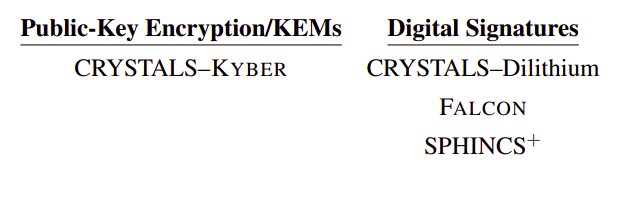
\includegraphics[width=.7\textwidth]{img/NISTround3.png}
	\caption{Algorithmes finalistes du round 3 à standardiser (voir \cite{NISTroundtrois})}
	\label{NISTround3}
\end{figure}

Bien qu'il reste des candidats à la standardisation dans le round 4, il semblerait que la cryptographie reposant sur les \hyperref[treillis]{treillis} soit le futur. En effet, Kyber et Dilithium, les deux algorithmes de la société CRYSTALS qui seront standardisés reposent sur la difficulté à résoudre un problème dans les treillis algébriques.\\

Dans le papier que CRYSTALS a envoyé au NIST (voir \cite{cristalslattice}) on nous présente vaguement le problème qui viendra remplacer le problème du logarithme discret (obsolète avec l'algorithme de Shor) dans les algorithmes post-quantiques. \\

En partant de ce problème simple où il suffit d'inverser $A$ et de multiplier par $z$ pour trouver le résultat (voir \ref{quantsimple})
\begin{figure}[h]
	\centering
	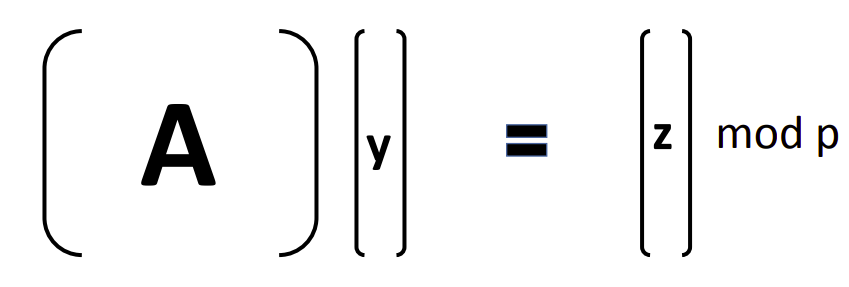
\includegraphics[width=\textwidth]{img/quantique_simple.png}
	\caption{Problème simple : connaissant $(A, z)$, trouver $y$}
	\label{quantsimple}
\end{figure}

Ils ont trouvé un problème bien plus dur à résoudre qui, s'il était facile, aurait plein d'applications non cryptographiques majeures (voir \ref{quantdur}).
\begin{figure}[h]
	\centering
	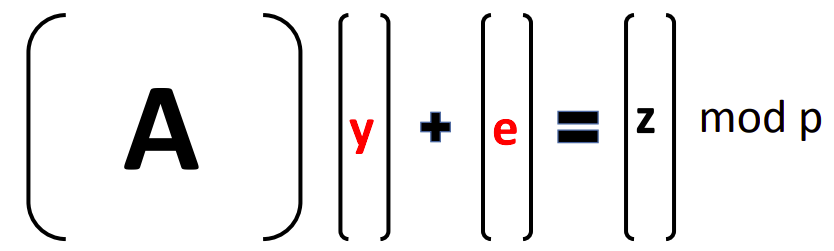
\includegraphics[width=\textwidth]{img/quantique_dur.png}
	\caption{Problème dur : connaissant $(A, z)$, trouver $(y, e)$}
	\label{quantdur}
\end{figure}
Ce problème est en effet un problème sur les treillis, car pour chaque paire $(y,e)$ on crée un nouveau treillis. Le problème illustré figure \ref{quantdur} en termes de treillis revient à trouver le point le plus proche de l'origine\footnote{Ce problème est aussi appelé problème BDD (Bilinear Diffie-Hellman)}.
\begin{figure}[h]
	\centering
	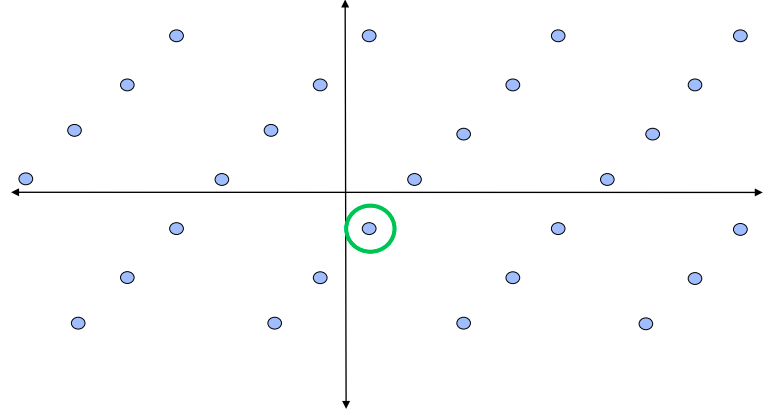
\includegraphics[width=\textwidth]{img/treilliIlu.png}
	\caption{Illustration d'un treillis issu du choix de $(y,e)$}
	\label{treilliIlu}
\end{figure}

L'intérêt de ce problème est que l'on ne connait pas encore d'algorithme (comme celui de Shor pour le problème du logarithme discret) qui permettrait de résoudre ce problème avec un ordinateur quantique. Par contre, on n'a pas non plus de preuve que ce genre de problème est réellement dur pour un ordinateur quantique (contrairement aux algorithmes symétriques). 

%\section{Le stage d'application dans la construction de mon projet professionel}

%Mon stage d'application au sein du groupe Thales a été une expérience cruciale qui a non seulement éclairé mes perceptions sur le fonctionnement d'un grand groupe, mais a également joué un rôle déterminant dans la définition de mon projet personnel. Au-delà de l'acquisition de compétences techniques, cette expérience m'a offert une compréhension approfondie de mes aspirations professionnelles et a orienté mes choix de carrière vers de nouveaux horizons. \\

%Chez Thales, j'ai pu apprécier la stabilité et le cadre structuré que propose un grand groupe. Cependant, j'ai également constaté que ces avantages sont souvent contrebalancés par une dynamique interne qui peut être relativement lente. Cette prise de conscience m'a amené à réfléchir sur la compatibilité de mon profil avec ce type d'environnement de travail.\\

%Mon expérience à Thales m'a conduit à une révélation importante : bien que je sois compétent en informatique, ma véritable passion ne réside pas dans la création d'applications ou la réécriture de solutions existantes. En revanche, j'ai découvert que c'est l'utilisation de l'informatique comme outil pour résoudre des problèmes complexes, similairement à ce que j'appréciais à l'école et en prépa, qui me motive vraiment. Cette distinction a été un tournant dans ma réflexion sur mon avenir professionnel.\\

%Mon stage m'a fait réaliser que mon intérêt pour les problèmes nouveaux et importants, ainsi que ma soif de théorie et de mathématiques, ne sont pas entièrement satisfaits dans le domaine de l'informatique appliquée. La cryptographie, bien qu'intéressante, m'a déçu par la relative rareté de l'application des mathématiques avancées dans la pratique. Cela m'a poussé à considérer des domaines plus théoriques comme la physique quantique.\\

%Bien que mon stage ait orienté mes aspirations loin de l'informatique d'application dans un grand groupe, il m'a également donné l'opportunité de rencontrer des professionnels influents. Ce réseau, bien qu'il ne corresponde peut-être pas directement à ma trajectoire actuelle, demeure une ressource précieuse pour l'avenir, offrant un appui potentiel si je devais un jour envisager une carrière dans un grand groupe français. 
\section{Conclusion}
En conclusion, ce stage d'application au sein de Thalès a été une expérience extrêmement enrichissante pour moi. J'ai pu approfondir mes connaissances en cryptographie, découvrir de nouveaux algorithmes et mettre en pratique mes compétences en programmation en Rust.\\

Ce stage m'a également permis de mieux définir mon projet professionnel. J'ai pu prendre conscience de la manière dont fonctionne un grand groupe et, plus particulièrement, de ce à quoi ressemble le métier d'ingénieur informatique dans ce contexte. \\J'ai aussi pu me rendre compte que mon penchant pour la recherche me fait préférer d'autres domaines que la cryptographie, et où les mathématiques sont plus présentes\footnote{comme la physique quantique par exemple}\footnote{Les mathématiques y sont la base de tout en cryptographie, mais en pratique et d'après l'expérience que j'ai eue, il n'y a qu'un petit nombre de chercheurs qui vont à la base des modèles et utilisent réellement les outils qui m'intéressent}. \\

Enfin, je tiens à remercier M. Mahmoud Chilali, mon tuteur, pour son accompagnement et ses conseils tout au long de ce stage. Je remercie également l'ensemble des employés de Thalès que j'ai pu rencontrer pour leur accueil chaleureux et leur disponibilité.
\printbibliography
\end{document}
